\documentclass[aspectratio=1610, professionalfonts, 13pt]{beamer}

% Lade das TU Dortund Theme von Max Nöthe
\usefonttheme[onlymath]{serif}
\usetheme[showtotalframes]{tudo}

% Lade richtiges Sprachpaket
\ifluatex
    \usepackage{polyglossia}
    \setmainlanguage{english}
\else
    \ifxetex
        \usepackage{polyglossia}
        \setmainlanguage{german}
    \else
        \usepackage[german]{babel}
    \fi
\fi

% Lade wichtige Mathematikpakete
\usepackage{amsmath}
\usepackage{amssymb}
\usepackage{mathtools}
\usepackage{cancel}
\usepackage[
  locale=DE,                   % deutsche Einstellungen
  separate-uncertainty=true,   % Immer Fehler mit \pm
  per-mode=symbol-or-fraction, % m/s im Text, sonst Brüche
]{siunitx}
\usepackage[absolute,overlay]{textpos}
\usepackage{framed}
\usepackage{multicol}
\usepackage{setspace}
\usepackage{graphicx}
\usepackage{booktabs}
\usepackage{caption}
\usepackage{appendixnumberbeamer}
\usepackage{tikz}
\usepackage[export]{adjustbox}
\usepackage{color}


% Lade Paket zur Nutzung von Schleifen
\usepackage{forloop}

% ------------------------- Präsentationsinformationen -------------------------

% Titel:
\title{\textbf{Tracker calibration studies in FairShip}}
\subtitle{SHiP}

% Autoren:
\author{Kevin Sedlaczek}

% Datum:
\date{July to September 2017}

% Lehrstuhl/Fakultät:
\institute[CERN]{Summer Student Programme}

% Titelgrafik:
\titlegraphic{
\includegraphics[width=0.2\textwidth]{logos/CERN-logo.jpg}\hfill
\includegraphics[width=0.2\textwidth]{logos/SHiP-Full_Black_0.png}}

% ------------------------------------------------------------------------------


\begin{document}

\maketitle

%-------------------------------INHALT EINFÜGEN---------------------------------

\begin{frame}[t]{content}
  \begin{enumerate} \setlength\itemsep{0.5cm}
    \item {\Large data sets}
    \item {\Large reconstructed distance to target}
    \item {\Large Monte Carlo truth and particle distribution}
    \item {\Large particle flux in strawtubes}
    %\item {\Large Ausblick}
  \end{enumerate}
\end{frame}

%------------------------------------------------------------------------------------------
\section{data sets}
%------------------------------------------------------------------------------------------
\begin{frame}[t]{Used data sets}
  \begin{itemize}
    \item Constructed via the FairShip framework
    \begin{itemize}
      \item \texttt{run\_SimScript.py} with flags \texttt{--MuonBack --FollowMuon} and \texttt{--Field} customized to change the field of the muon shield.
      \item \texttt{ShipReco.py} to simulate the reconstruction and detector
      \item files with different magnetic fields \texttt{muShield.B} of the muon shield
      \item And also without any magnetic field in all detector components (\texttt{c.tauMS.B}$=\SI{1.5}{\tesla}$/\texttt{c.EmuMagnet.B}$=\SI{1}{\tesla}$)
      \item first samples with 100\,000 events
      \item use of weights for certain events
    \end{itemize}
  \end{itemize}
\end{frame}

\begin{frame}[t]{The detector}
  \begin{figure}
    \centering
    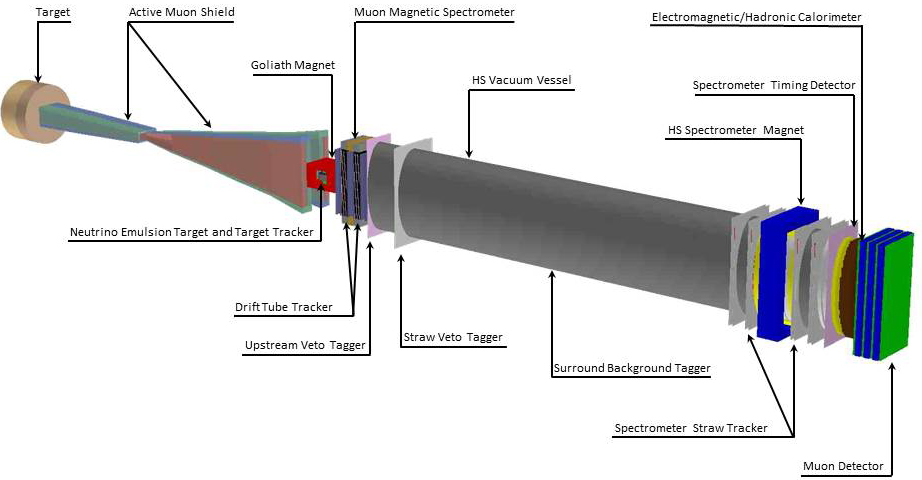
\includegraphics[width=0.8\textwidth]{tpdetector.jpg}
  \end{figure}
\end{frame}

%------------------------------------------------------------------------------------------
\section{Target IP}
%------------------------------------------------------------------------------------------


%\begin{frame}[t]{reconstructed distances to the target}
%  \begin{itemize}
%    \item possible to use reconstructed coordinates at target as a selection criterium?
%    \item real production vertex in MC truth
%    \item reconstructed tracks offer momenta of particles at certain points in the detector
%    \item one can use this information to linearly extrapolate back to the target z-postion
%  \end{itemize}
%\end{frame}


\begin{frame}[t]{Calculation of impact parameter}
    The reconstructed tracks (namely the fitted states) are accessed via:
    \begin{figure}
      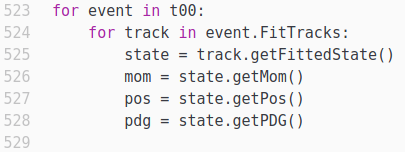
\includegraphics[width=0.4\textwidth,left]{loop.png}
    \end{figure}
    They yield a spatial vector $\vec{r}_\text{track}=(x,y,z)$ and a momentum vector $(p_x,p_y,p_z)$. The spatial vector is used as a starting point, while the momentum vector defines the direction. The so defined straight line in 3D space can then be extrapolated to the z-component of the target centre.
\end{frame}

\begin{frame}[t]{}
  \begin{multicols}{2}
    \begin{figure}
      \centering
      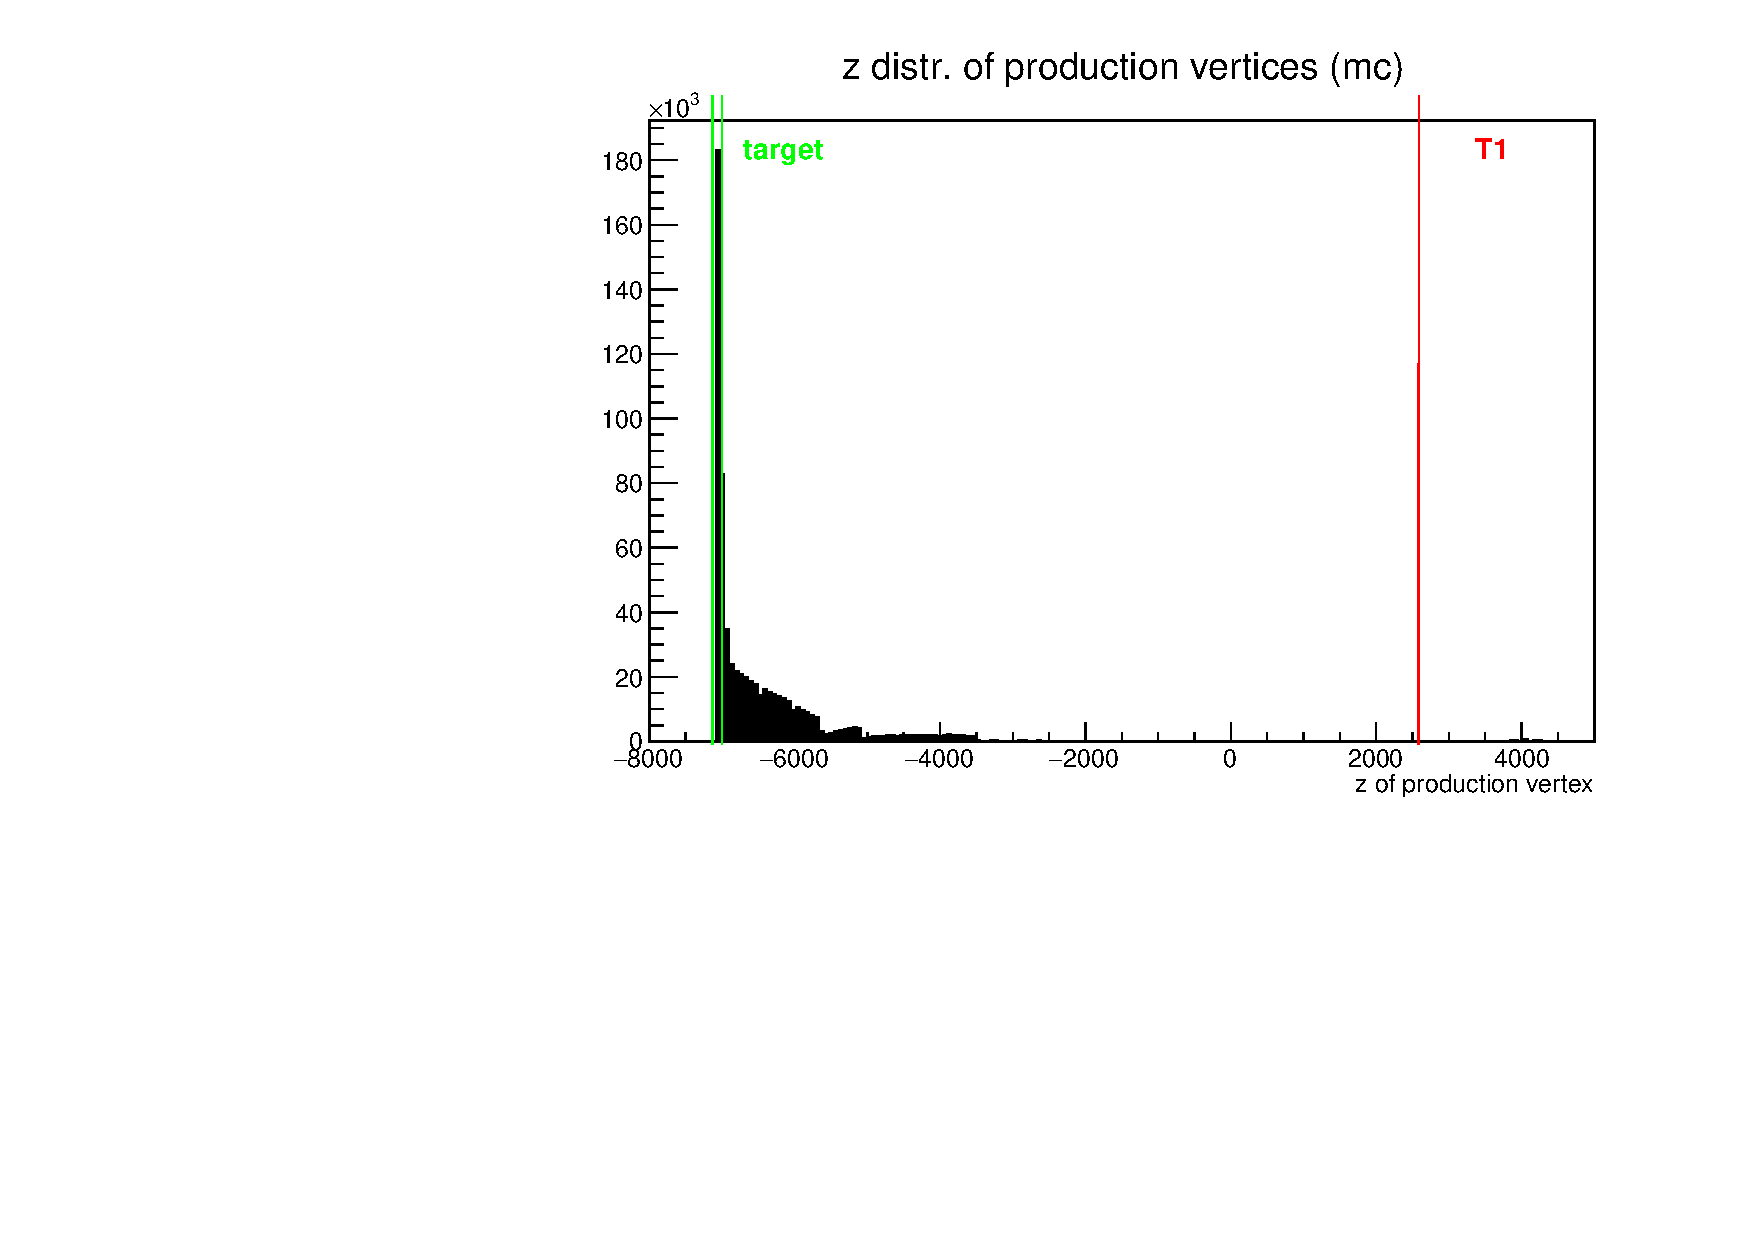
\includegraphics[width=0.5\textwidth]{../hists/nofield/mc_pvtx_z.pdf}
    \end{figure}
    \columnbreak
    \begin{figure}
      \centering
      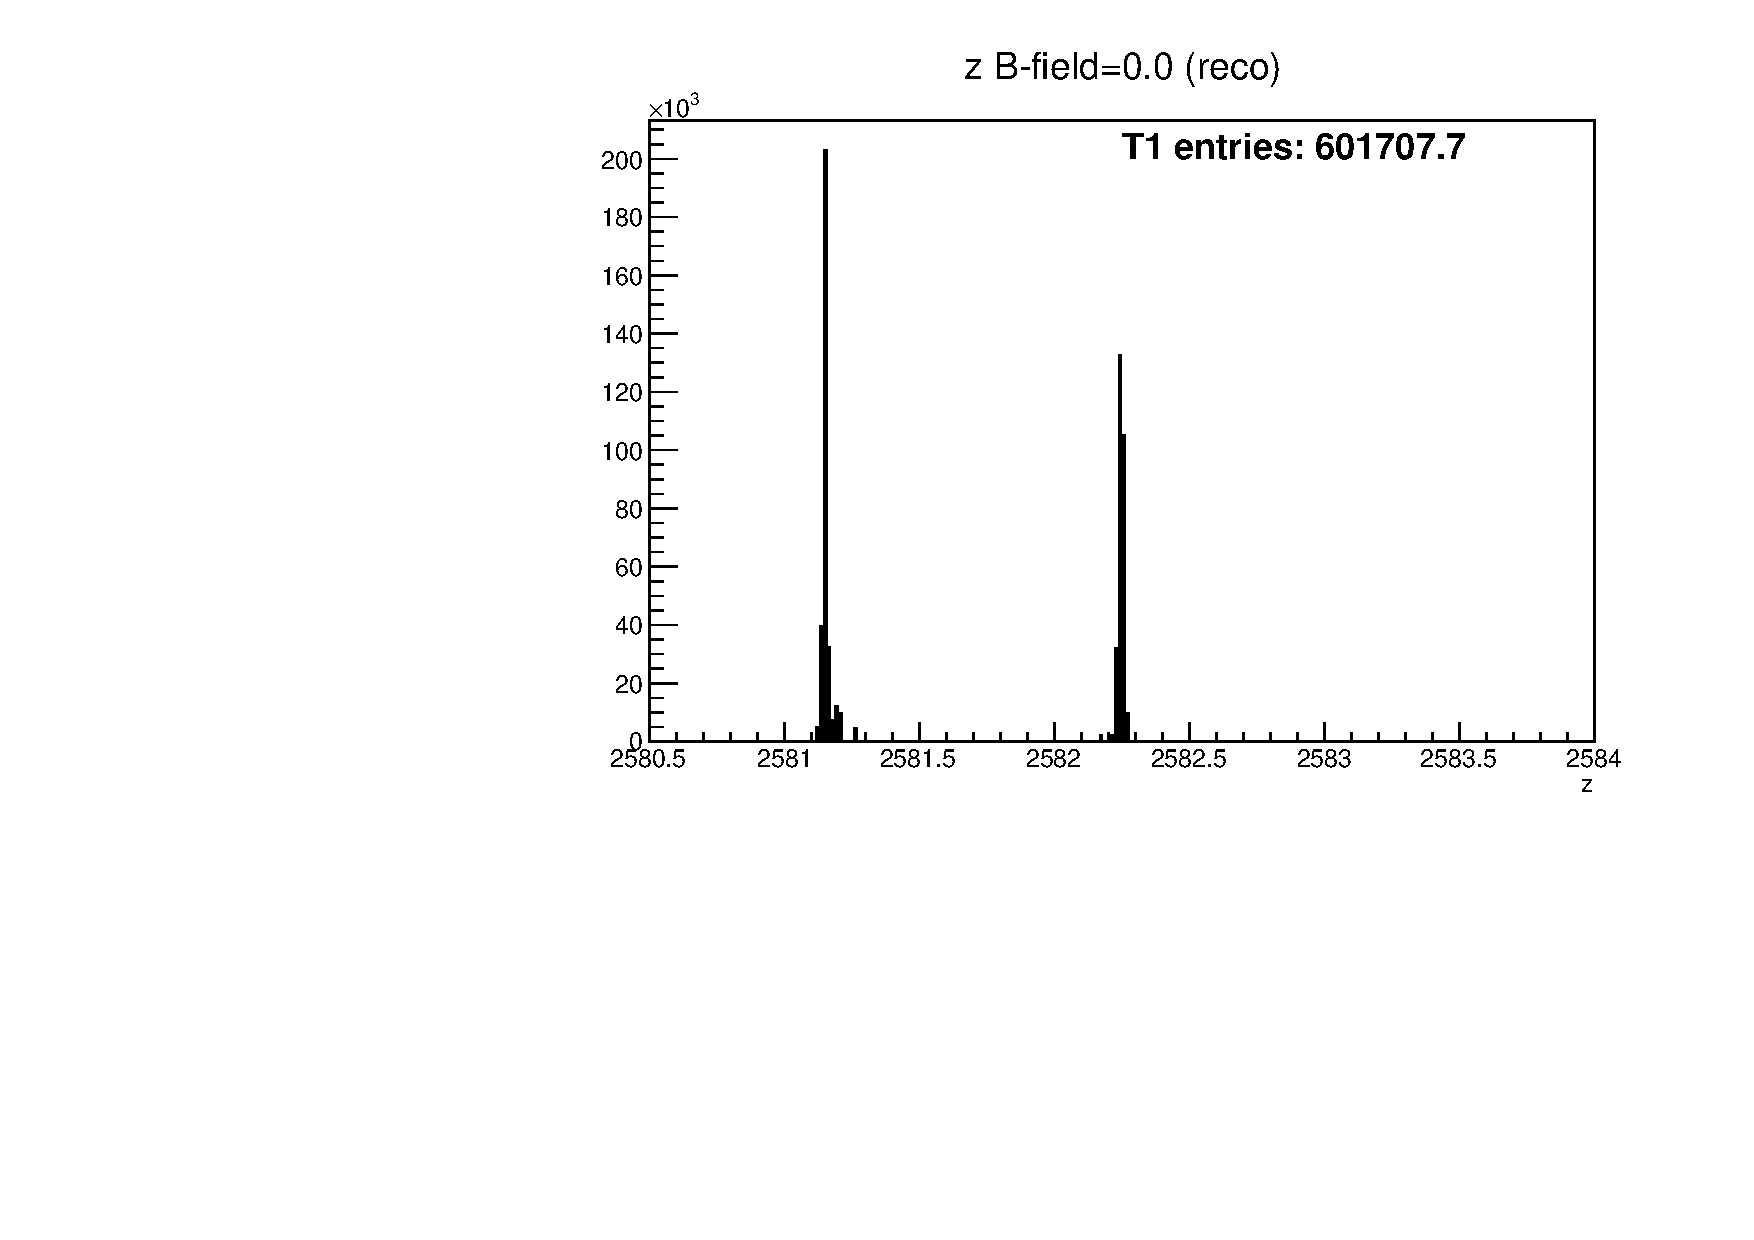
\includegraphics[width=0.5\textwidth]{../hists/nofield/z_500k.pdf}
    \end{figure}
  \end{multicols}
\end{frame}

\begin{frame}[t]{Calculation of impact parameter}
  The target centre is located at $z_t=-7067.0$, so that the $x$ and $y$ coordinates of the fitted tracks can be calculated. Of course assuming there is no scattering and no magnetic field altering the direction of the momentum of the particles. So the track is described by
  %
  \begin{equation}
    \vec{r}(t)=\vec{p}\cdot t+\vec{r}_\text{track}
  \end{equation}
  Thus one only needs to calculate the $t$ for the $z$-component and apply it to $x$ and $y$.
  \begin{itemize}
    \item $t = \frac{z_\text{target}-z}{p_z}$
    \item $x_\text{target} = p_x\cdot t + x$
    \item $y_\text{target} = p_y\cdot t + y$
    \item this then gives the distance in the $x$-$y$-plain: $d = \sqrt{x_\text{target}^2+y_\text{target}^2}$
  \end{itemize}
\end{frame}

\begin{frame}[t]{}
  \begin{figure}
    \centering
    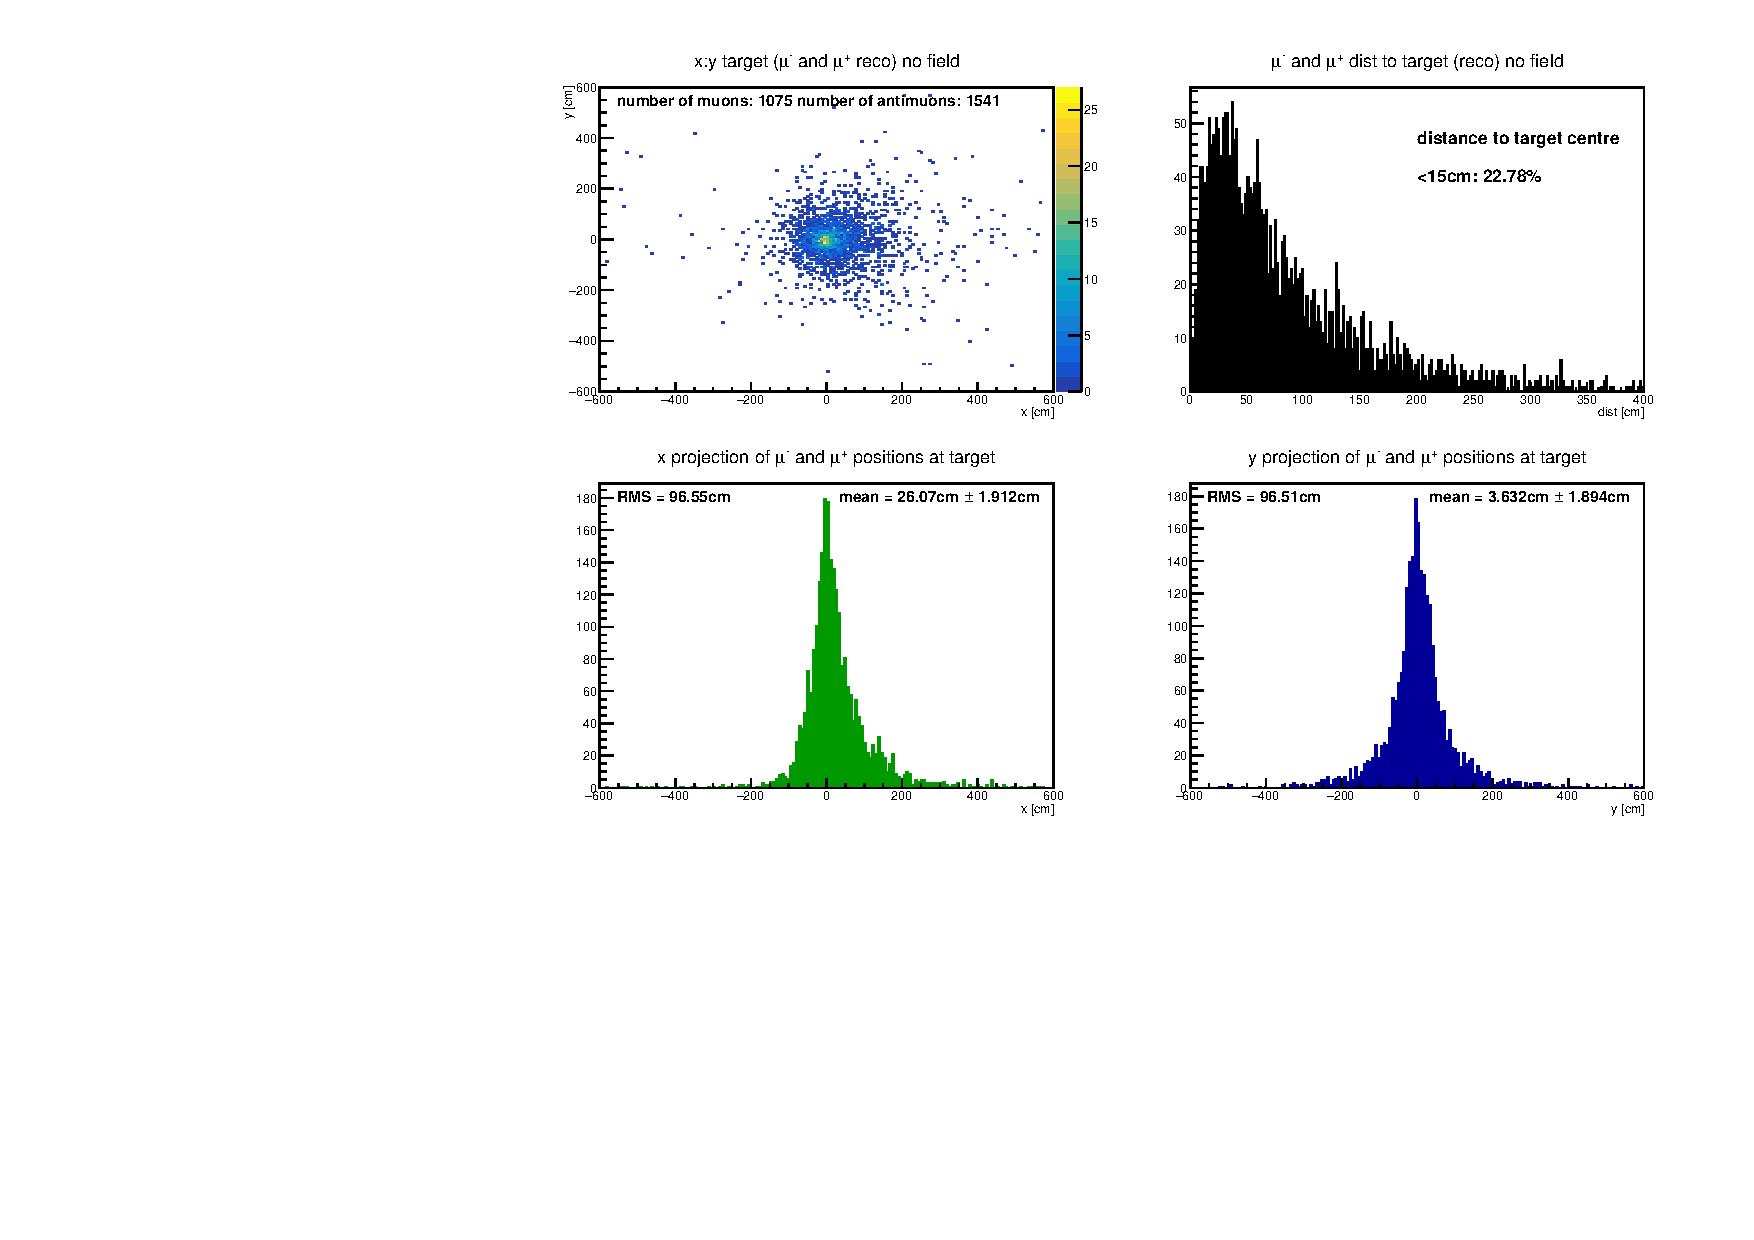
\includegraphics[width=0.65\textwidth]{../hists/nofield/target_dist.pdf}
  \end{figure}
\end{frame}

\begin{frame}[t]{Divided for $\mu^+$ and $\mu^-$}
  \begin{multicols}{2}
    \begin{figure}
      \centering
      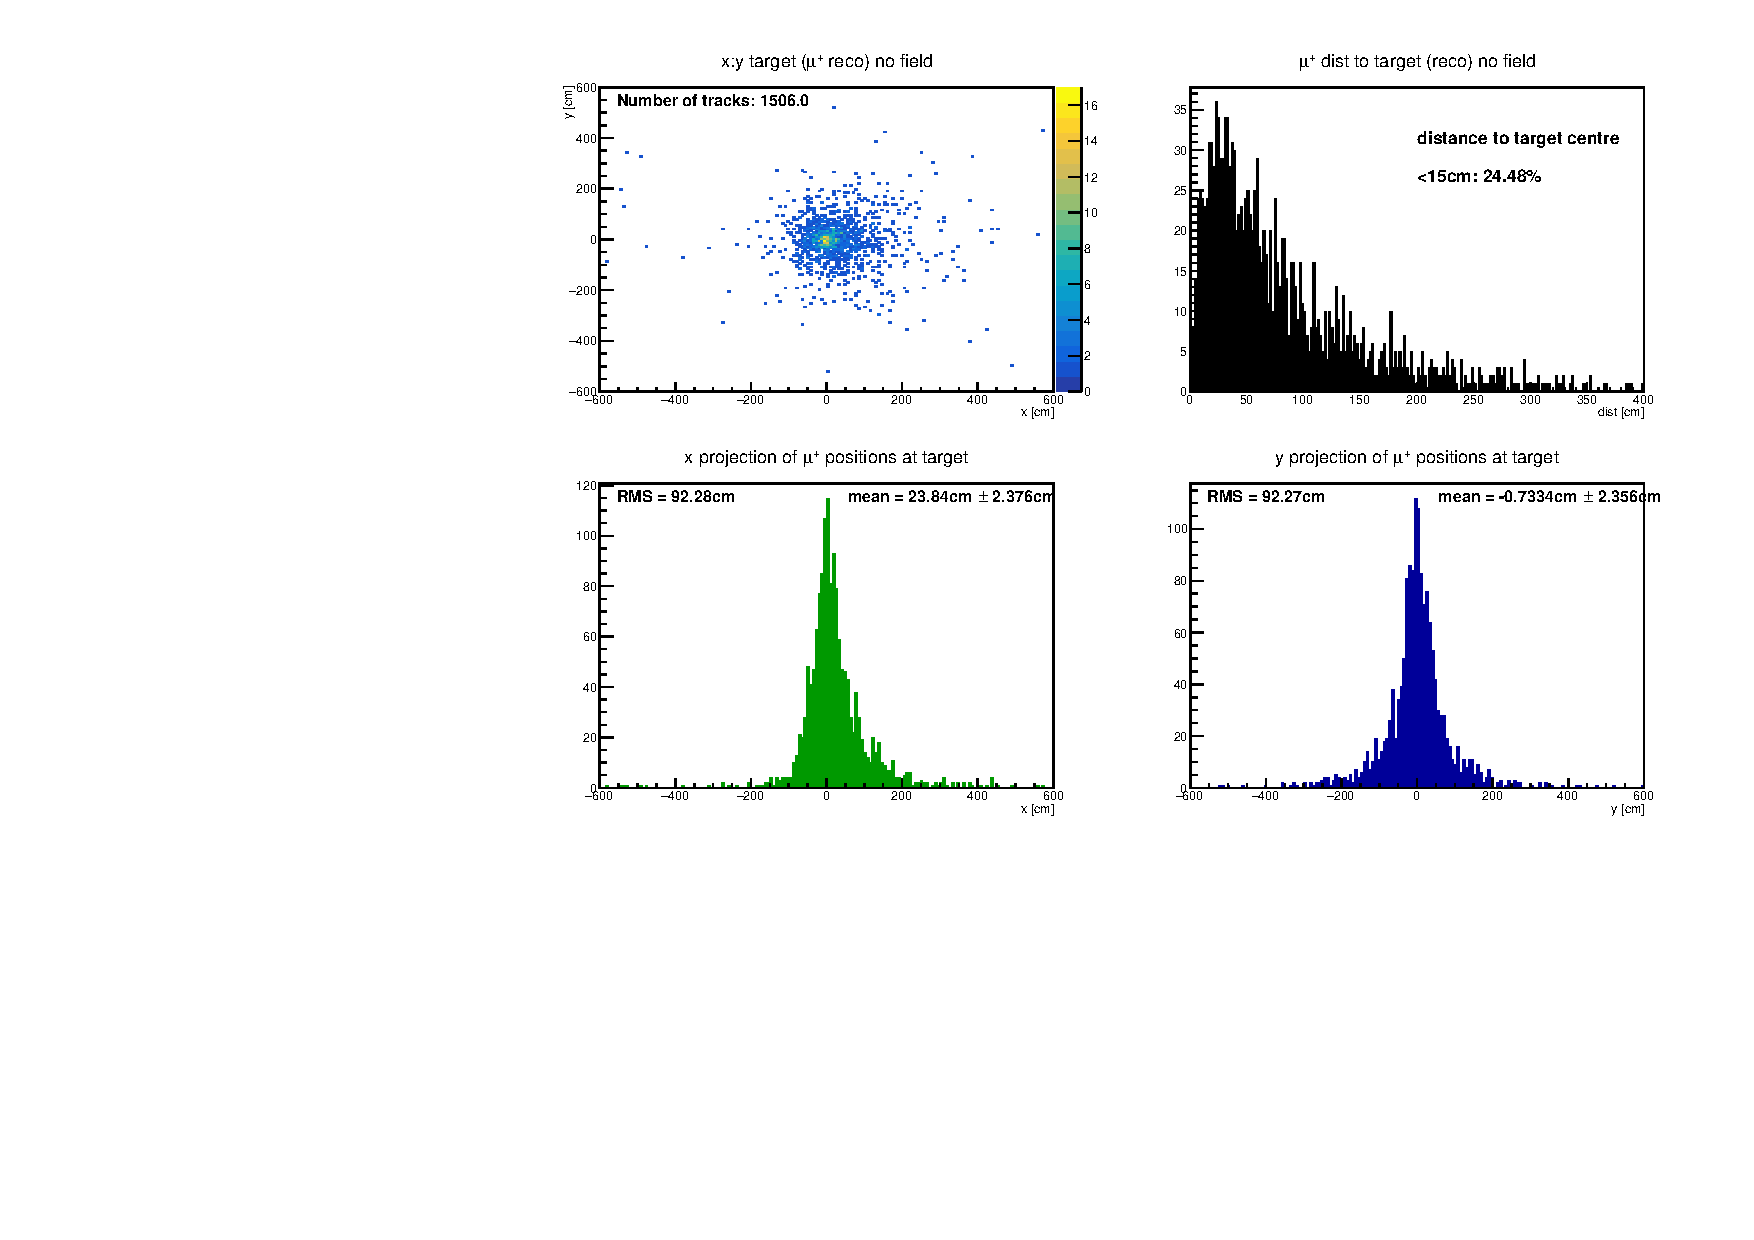
\includegraphics[width=0.5\textwidth]{../hists/nofield/allP/target_dist_amu.pdf}
    \end{figure}
    \columnbreak
    \begin{figure}
      \centering
      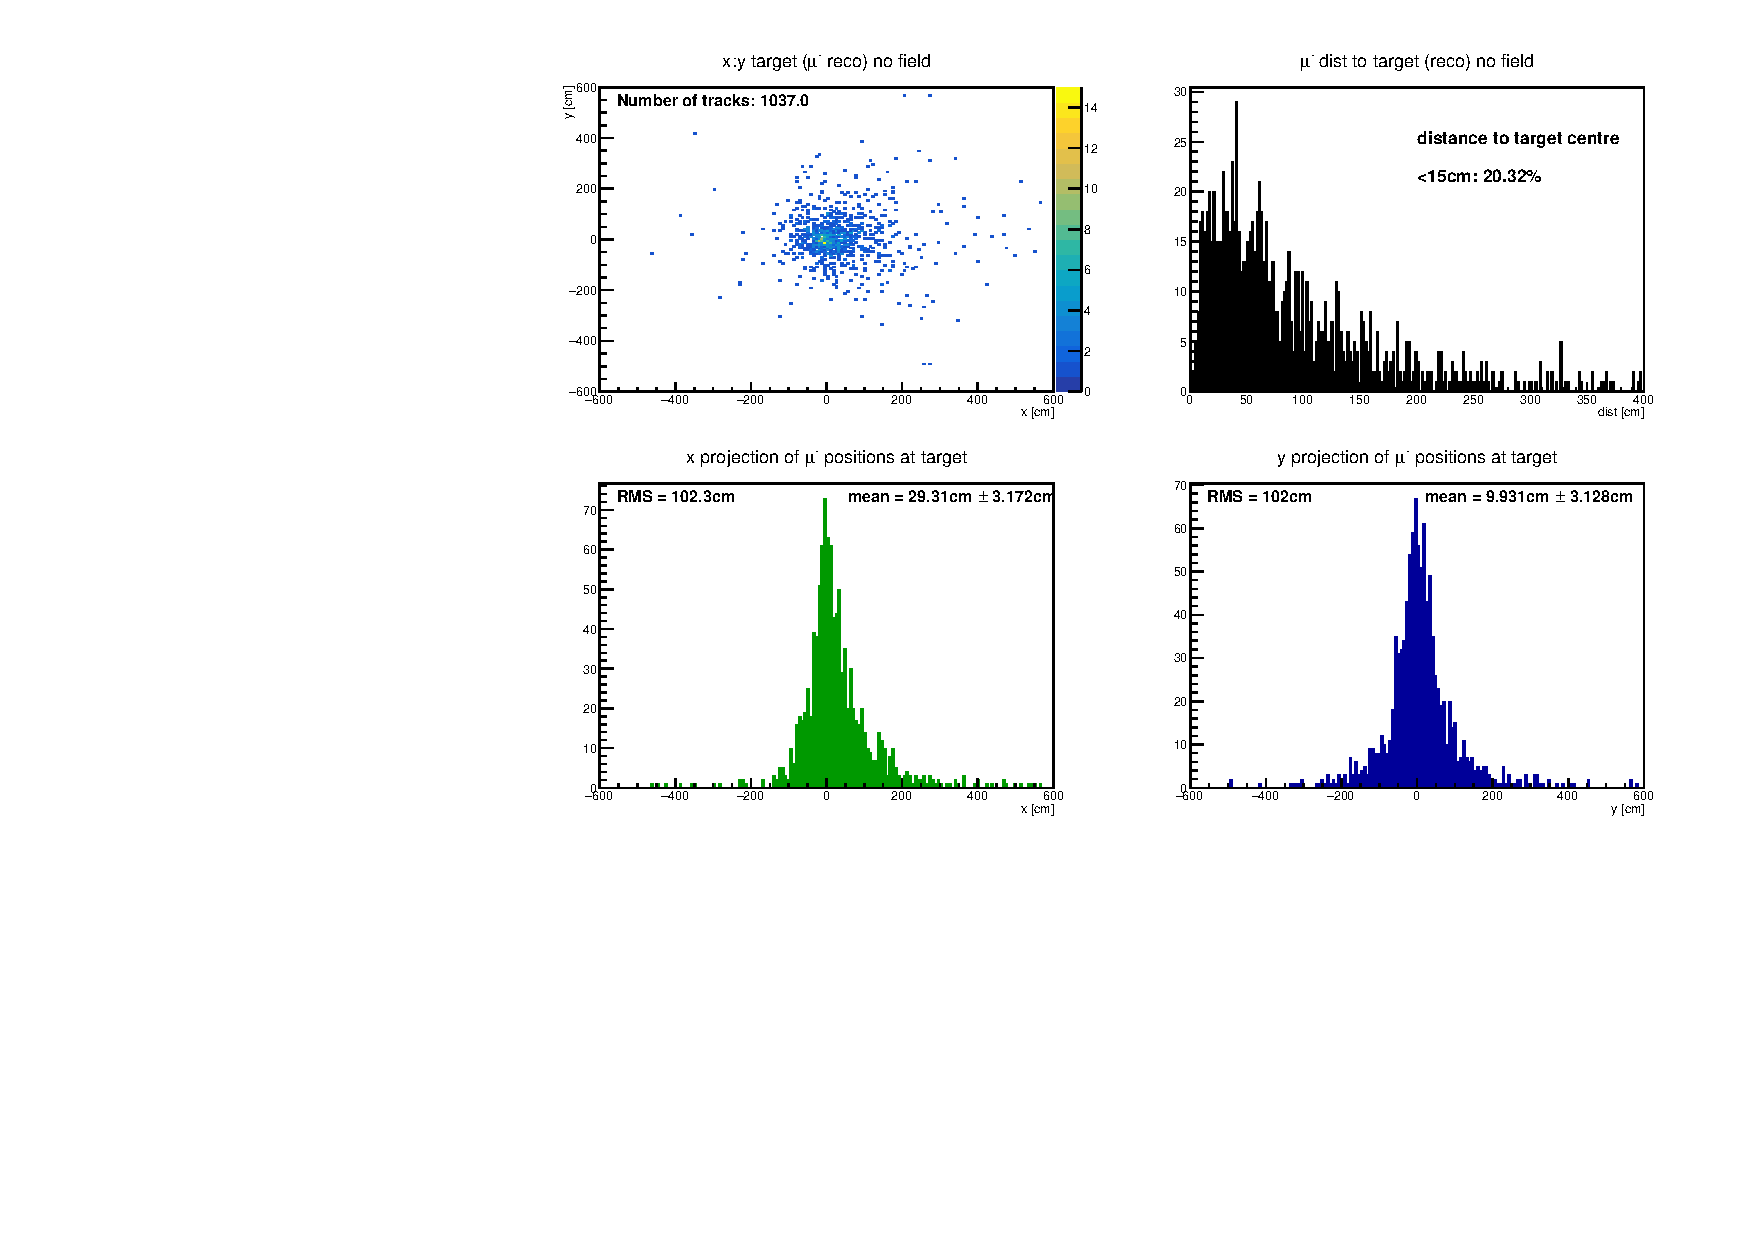
\includegraphics[width=0.5\textwidth]{../hists/nofield/allP/target_dist_mu.pdf}
    \end{figure}
  \end{multicols}
\end{frame}

\begin{frame}[t]{Momentum distribution of the tracks}
  \begin{figure}
    \centering
    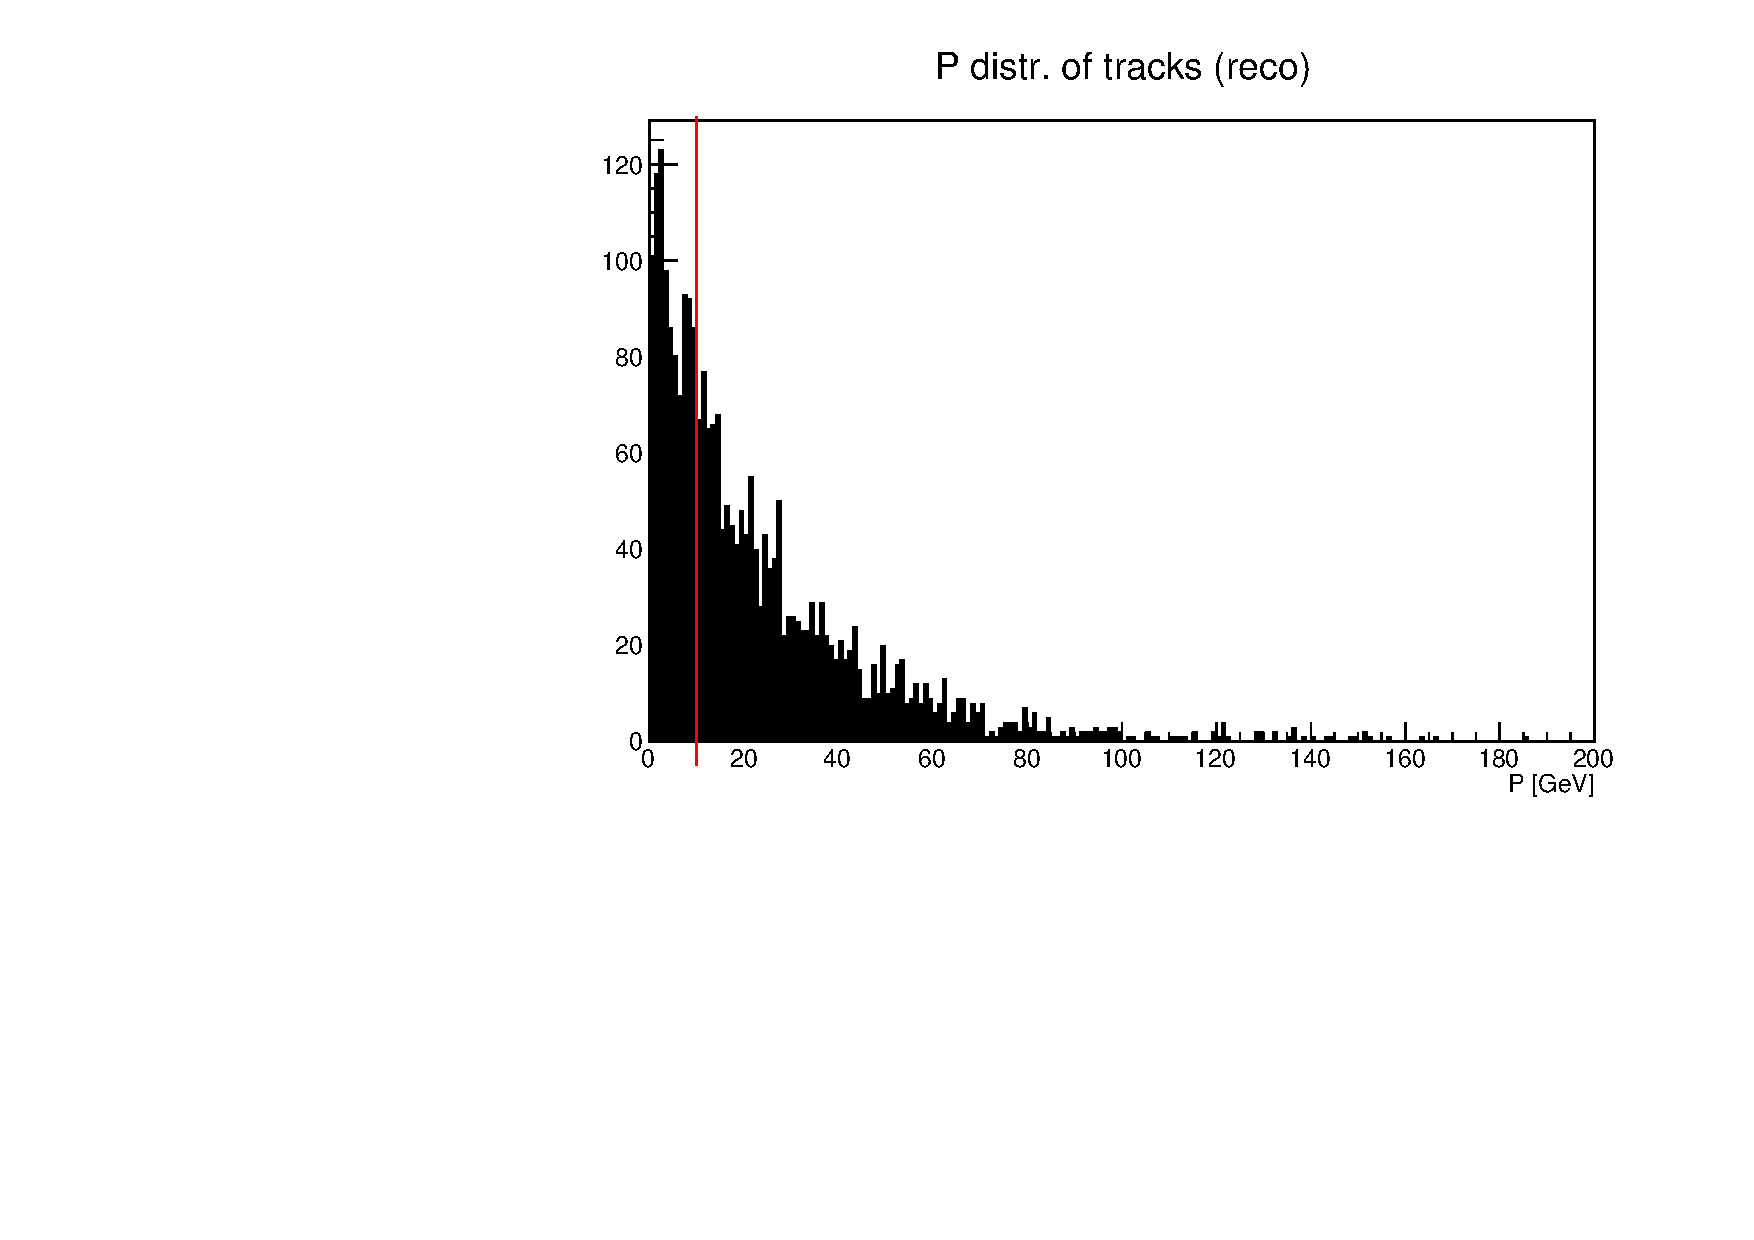
\includegraphics[width=0.65\textwidth]{../hists/nofield/mom_reco_tracks.pdf}
  \end{figure}
\end{frame}

\begin{frame}[t]{Divided for $\mu^+$ and $\mu^-$ only momenta $> \SI{10}{\giga\electronvolt}$}
  \begin{multicols}{2}
    \begin{figure}
      \centering
      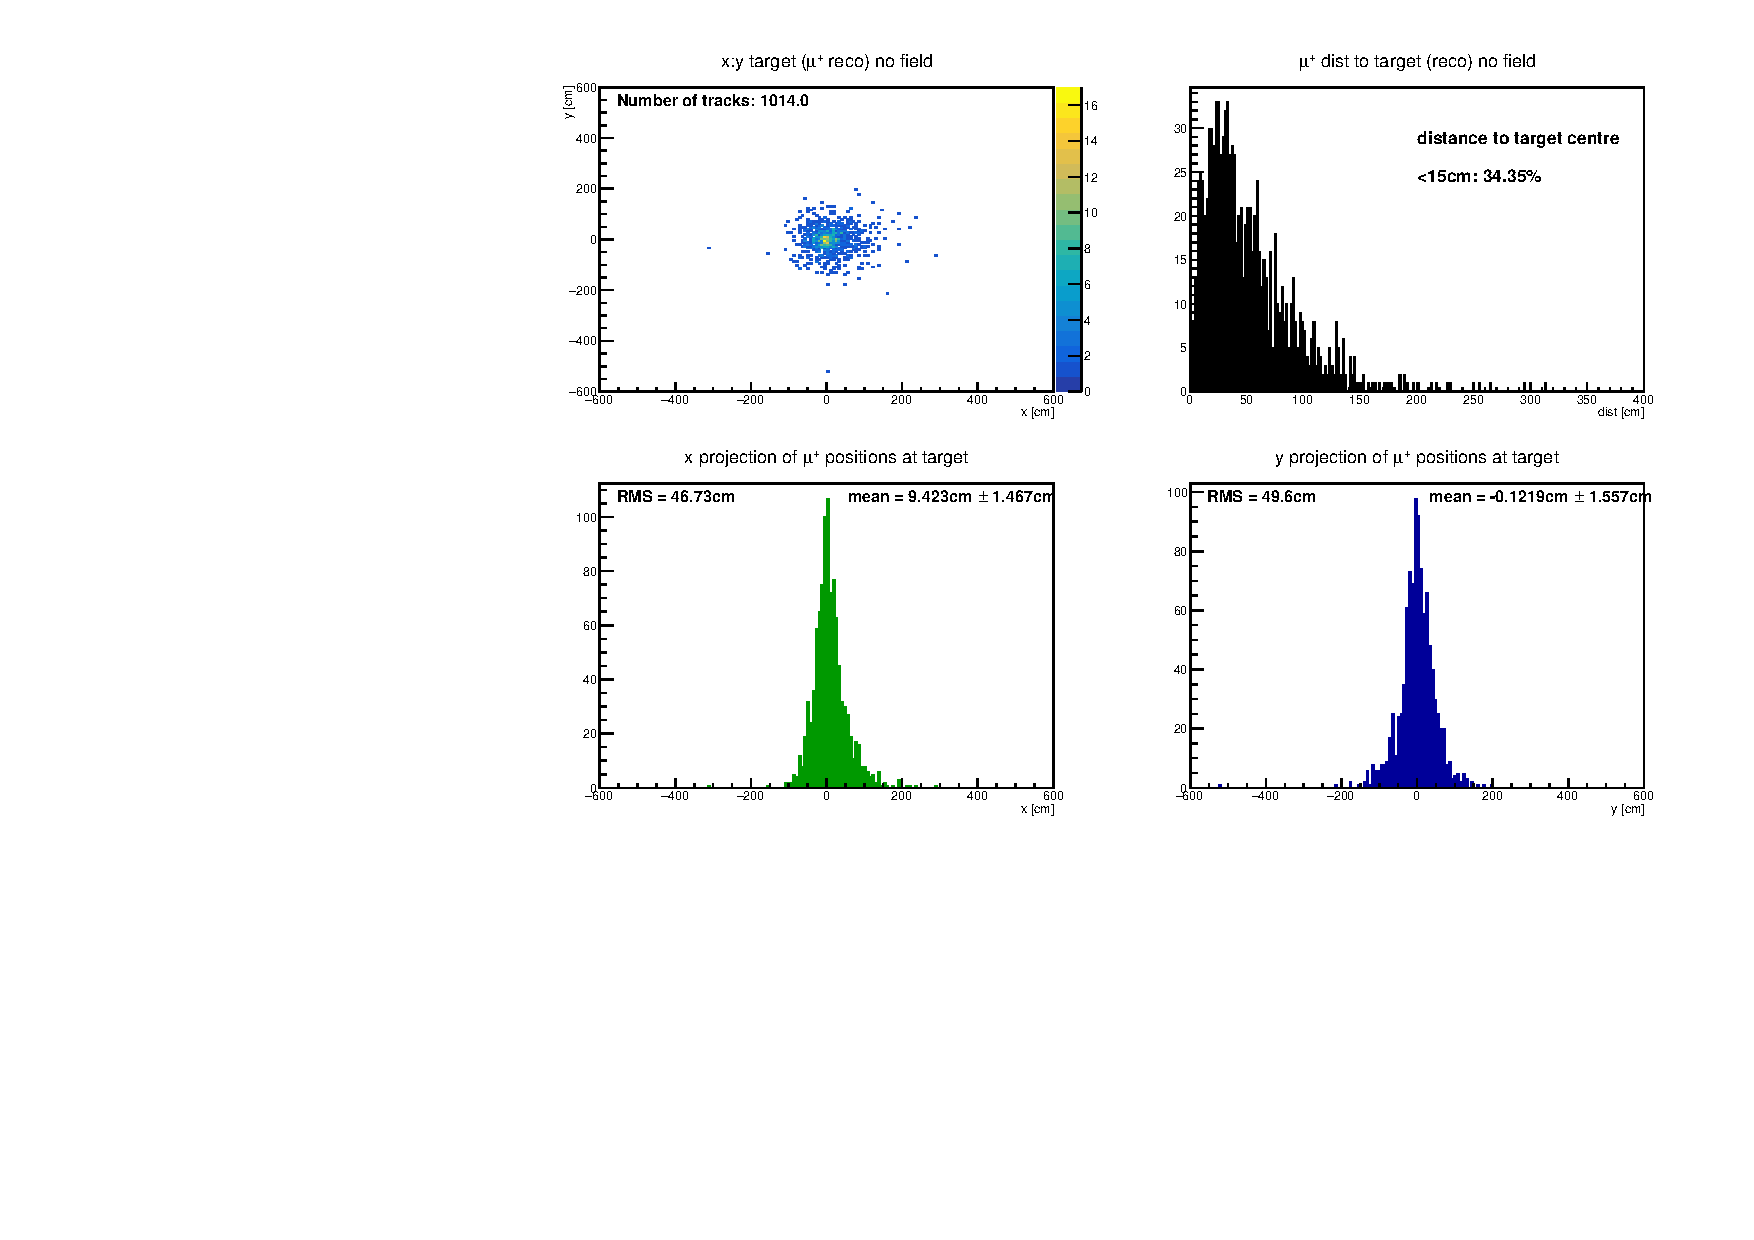
\includegraphics[width=0.5\textwidth]{../hists/nofield/P/target_dist_amu.pdf}
    \end{figure}
    \columnbreak
    \begin{figure}
      \centering
      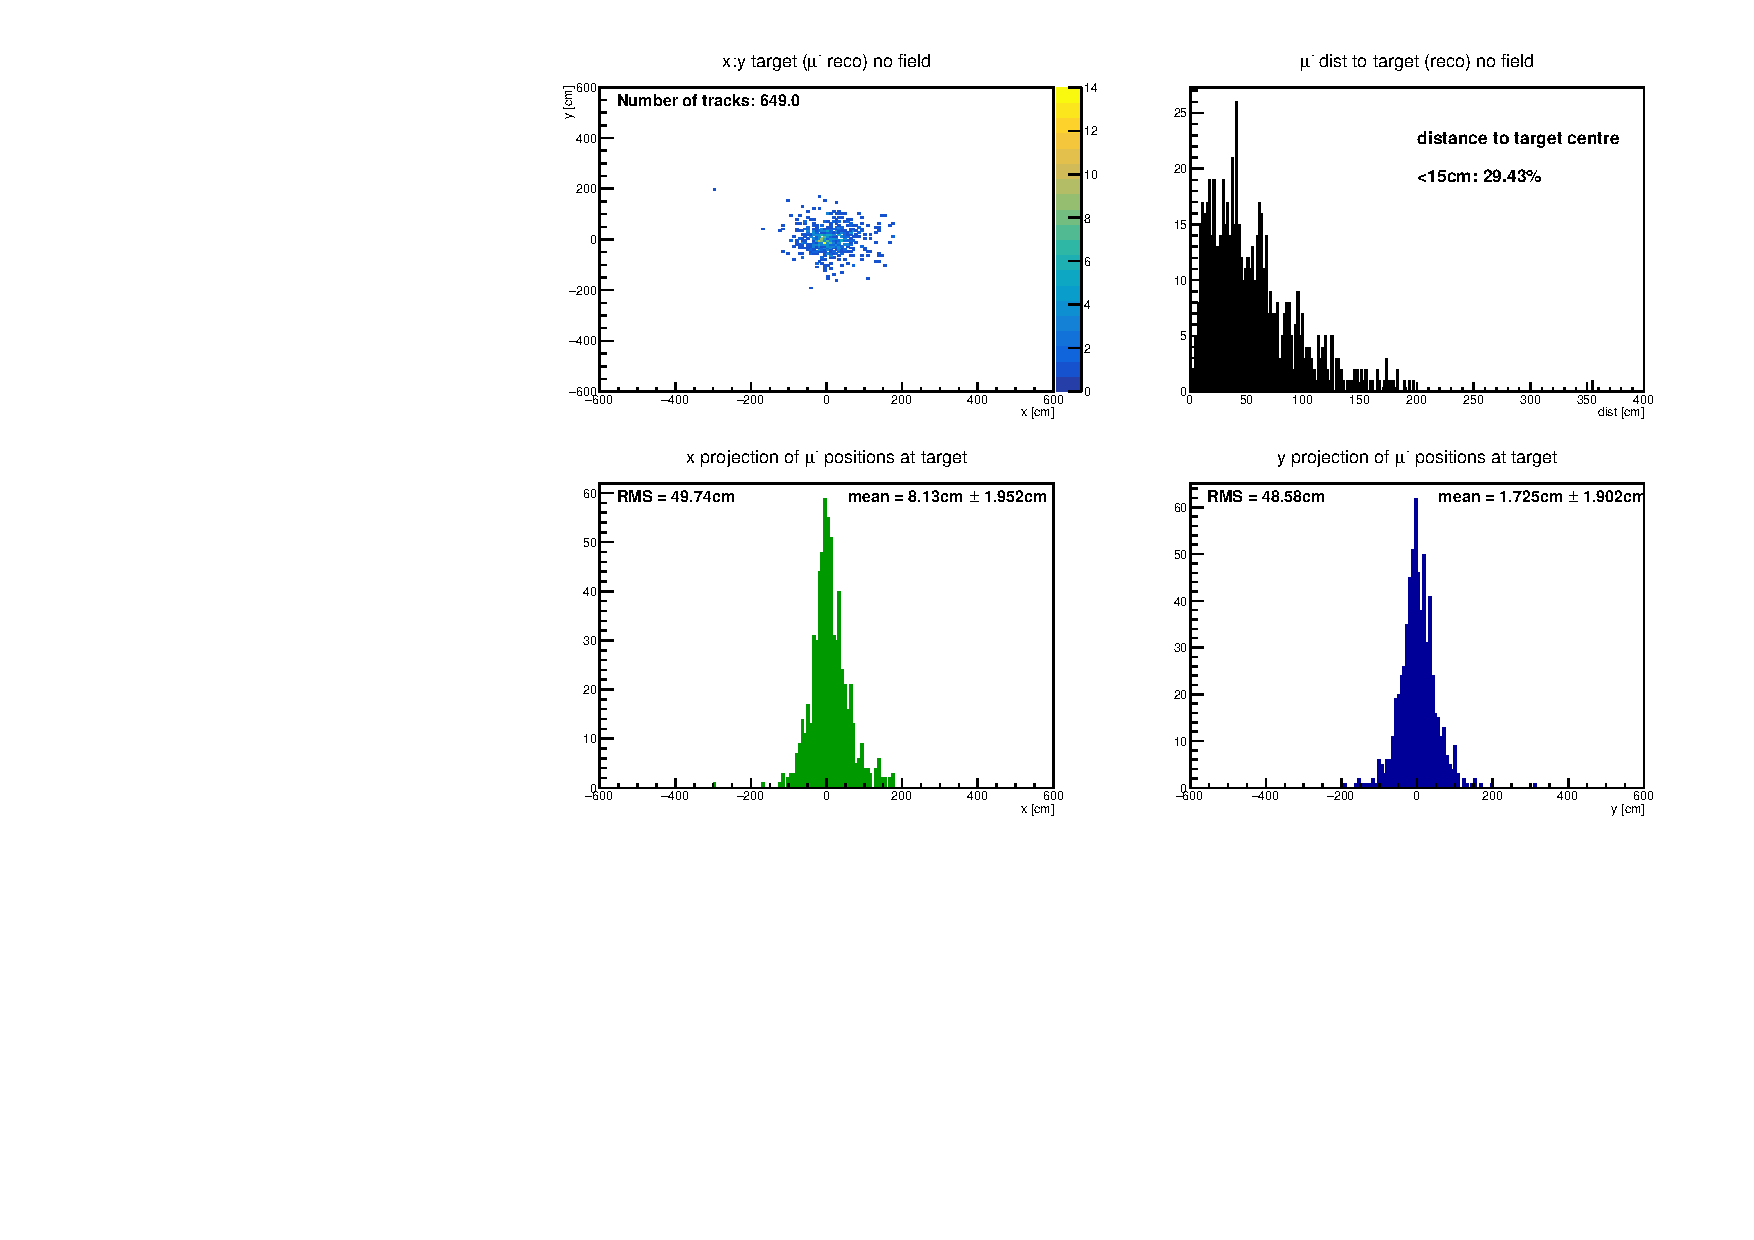
\includegraphics[width=0.5\textwidth]{../hists/nofield/P/target_dist_mu.pdf}
    \end{figure}
  \end{multicols}
\end{frame}

\begin{frame}[t]{Divided for $\mu^+$ and $\mu^-$ only momenta $< \SI{10}{\giga\electronvolt}$}
  \begin{multicols}{2}
    \begin{figure}
      \centering
      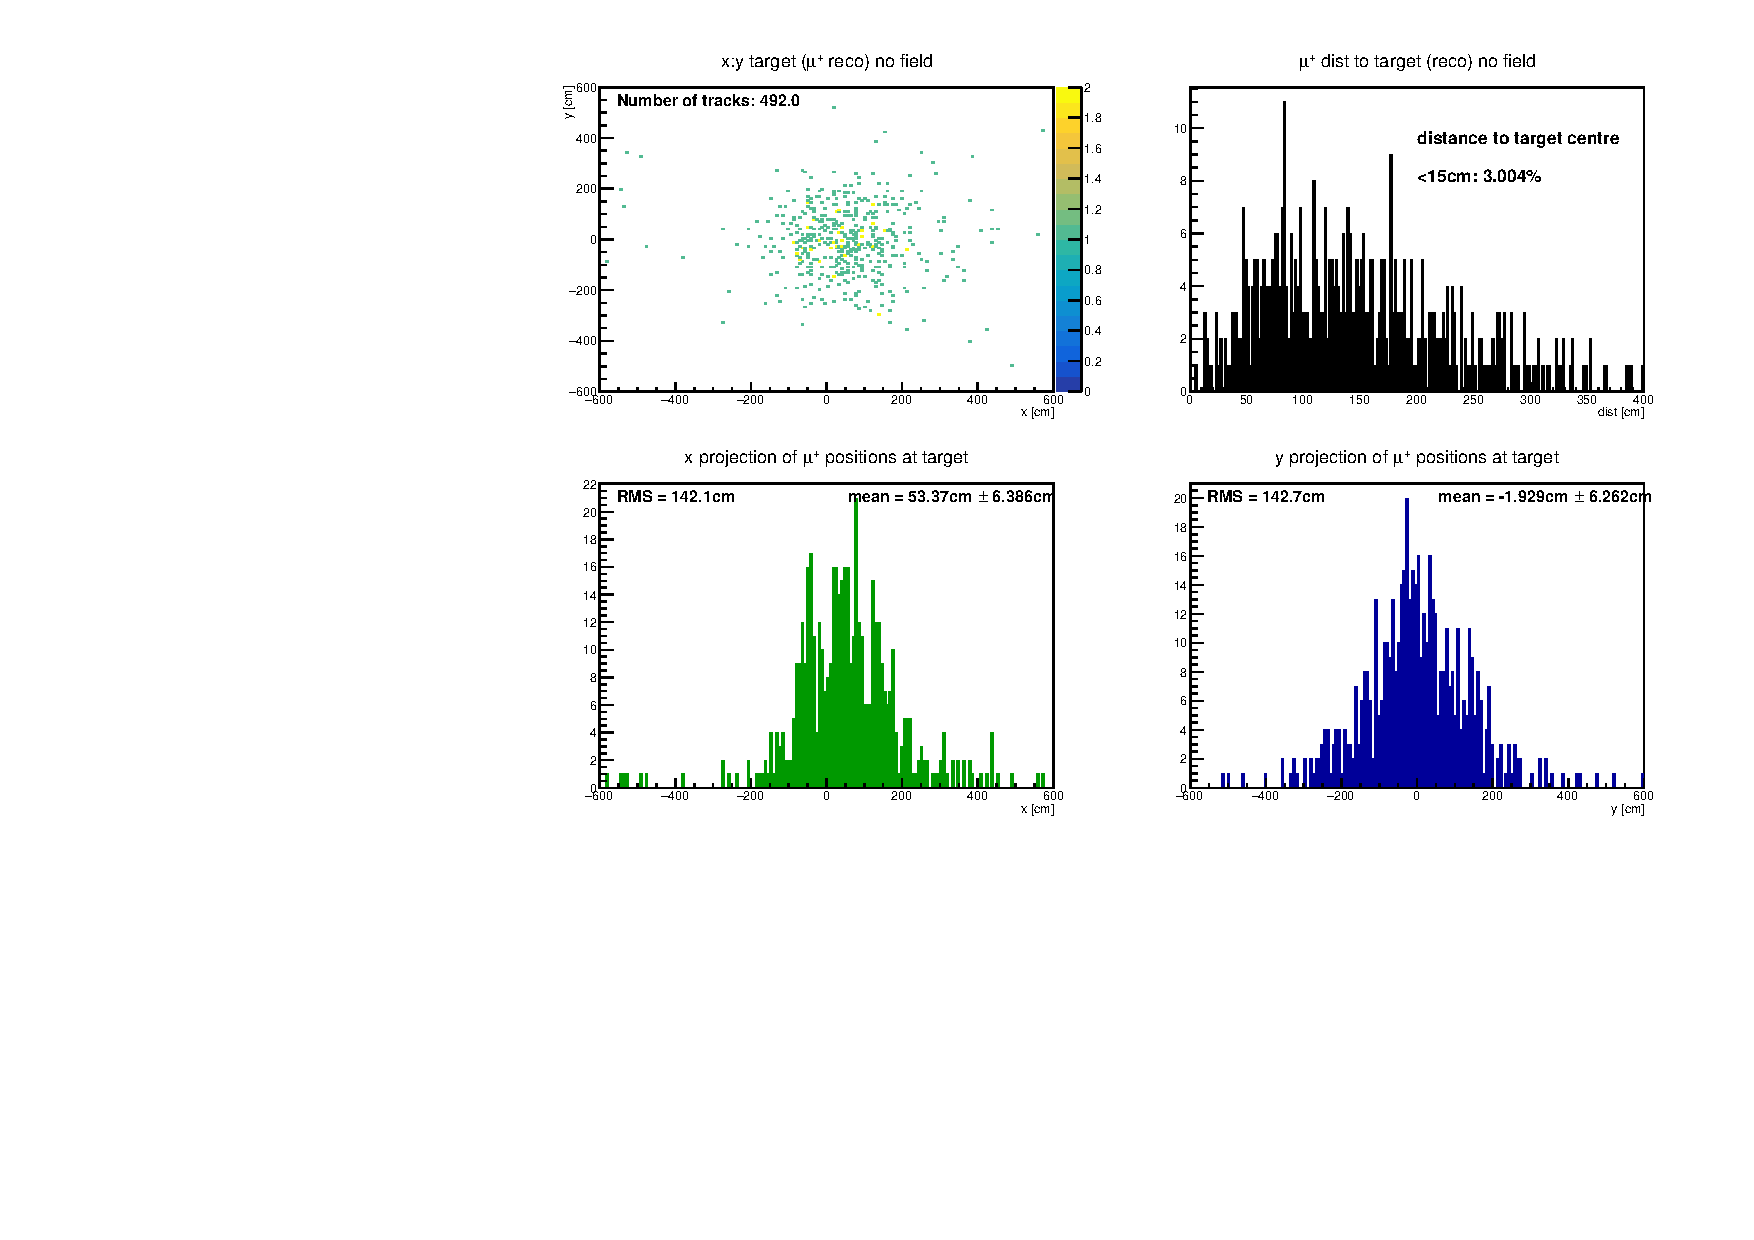
\includegraphics[width=0.5\textwidth]{../hists/nofield/p/target_dist_amu.pdf}
    \end{figure}
    \columnbreak
    \begin{figure}
      \centering
      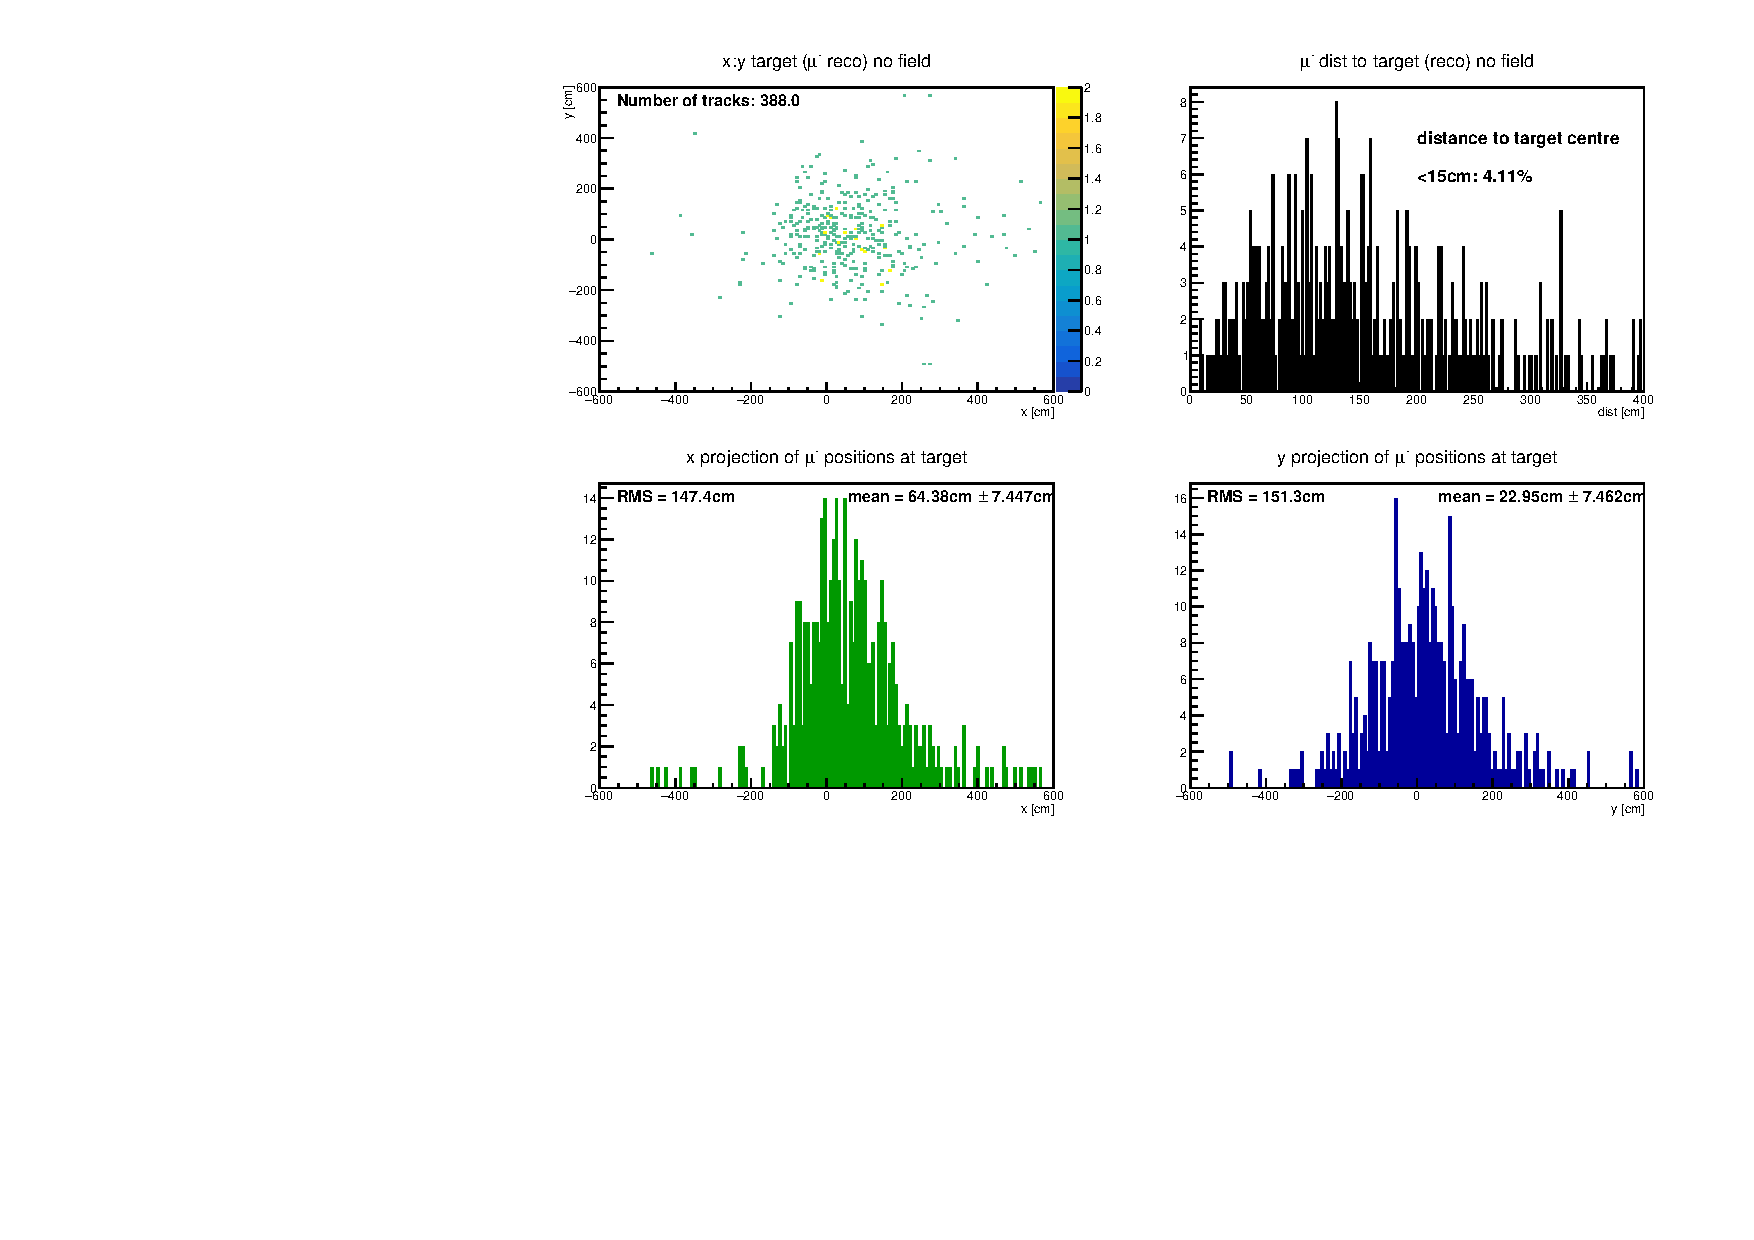
\includegraphics[width=0.5\textwidth]{../hists/nofield/p/target_dist_mu.pdf}
    \end{figure}
  \end{multicols}
\end{frame}

\begin{frame}
  \begin{table}
    \centering
    \begin{tabular}{c
                    S
                    S
                    S}
      \toprule
      {$\mu^{+}$} & {all momenta} & {$p>\SI{10}{\giga\electronvolt}$} & {$p<\SI{10}{\giga\electronvolt}$} \\
      \midrule
      mean $x$ /cm & 23.84(238) & 9.4(15) & 53.37(639) \\
      mean $y$ /cm & -0.733(2356) & -0.12(156) & -1.93(626) \\
      RMS $x$ /cm & 92.28 & 46.73 & 142.1 \\
      RMS $y$ /cm & 92.27 & 49.6 & 142.7 \\
      \midrule
      {$\mu^{-}$} & {all momenta} & {$p>\SI{10}{\giga\electronvolt}$} & {$p<\SI{10}{\giga\electronvolt}$} \\
      \midrule
      mean $x$ /cm & 29.31(317) & 8.13(195) & 64.38(745)  \\
      mean $y$ /cm & 9.931(3128) & 1.725(1902) & 22.95(746)  \\
      RMS $x$ /cm & 102.3 & 49.74 & 147.4  \\
      RMS $y$ /cm & 102 & 48.58 & 151.3  \\
      \bottomrule
    \end{tabular}
    \caption{Means and RMS of the $x$- and $y$-projections of the reconstructed IP.}
    \label{tab:mean}
  \end{table}
\end{frame}

\begin{frame}[t]{Divided for $\mu^+$ and $\mu^-$ all momenta but muon shield 1mT}
  \begin{multicols}{2}
    \begin{figure}
      \centering
      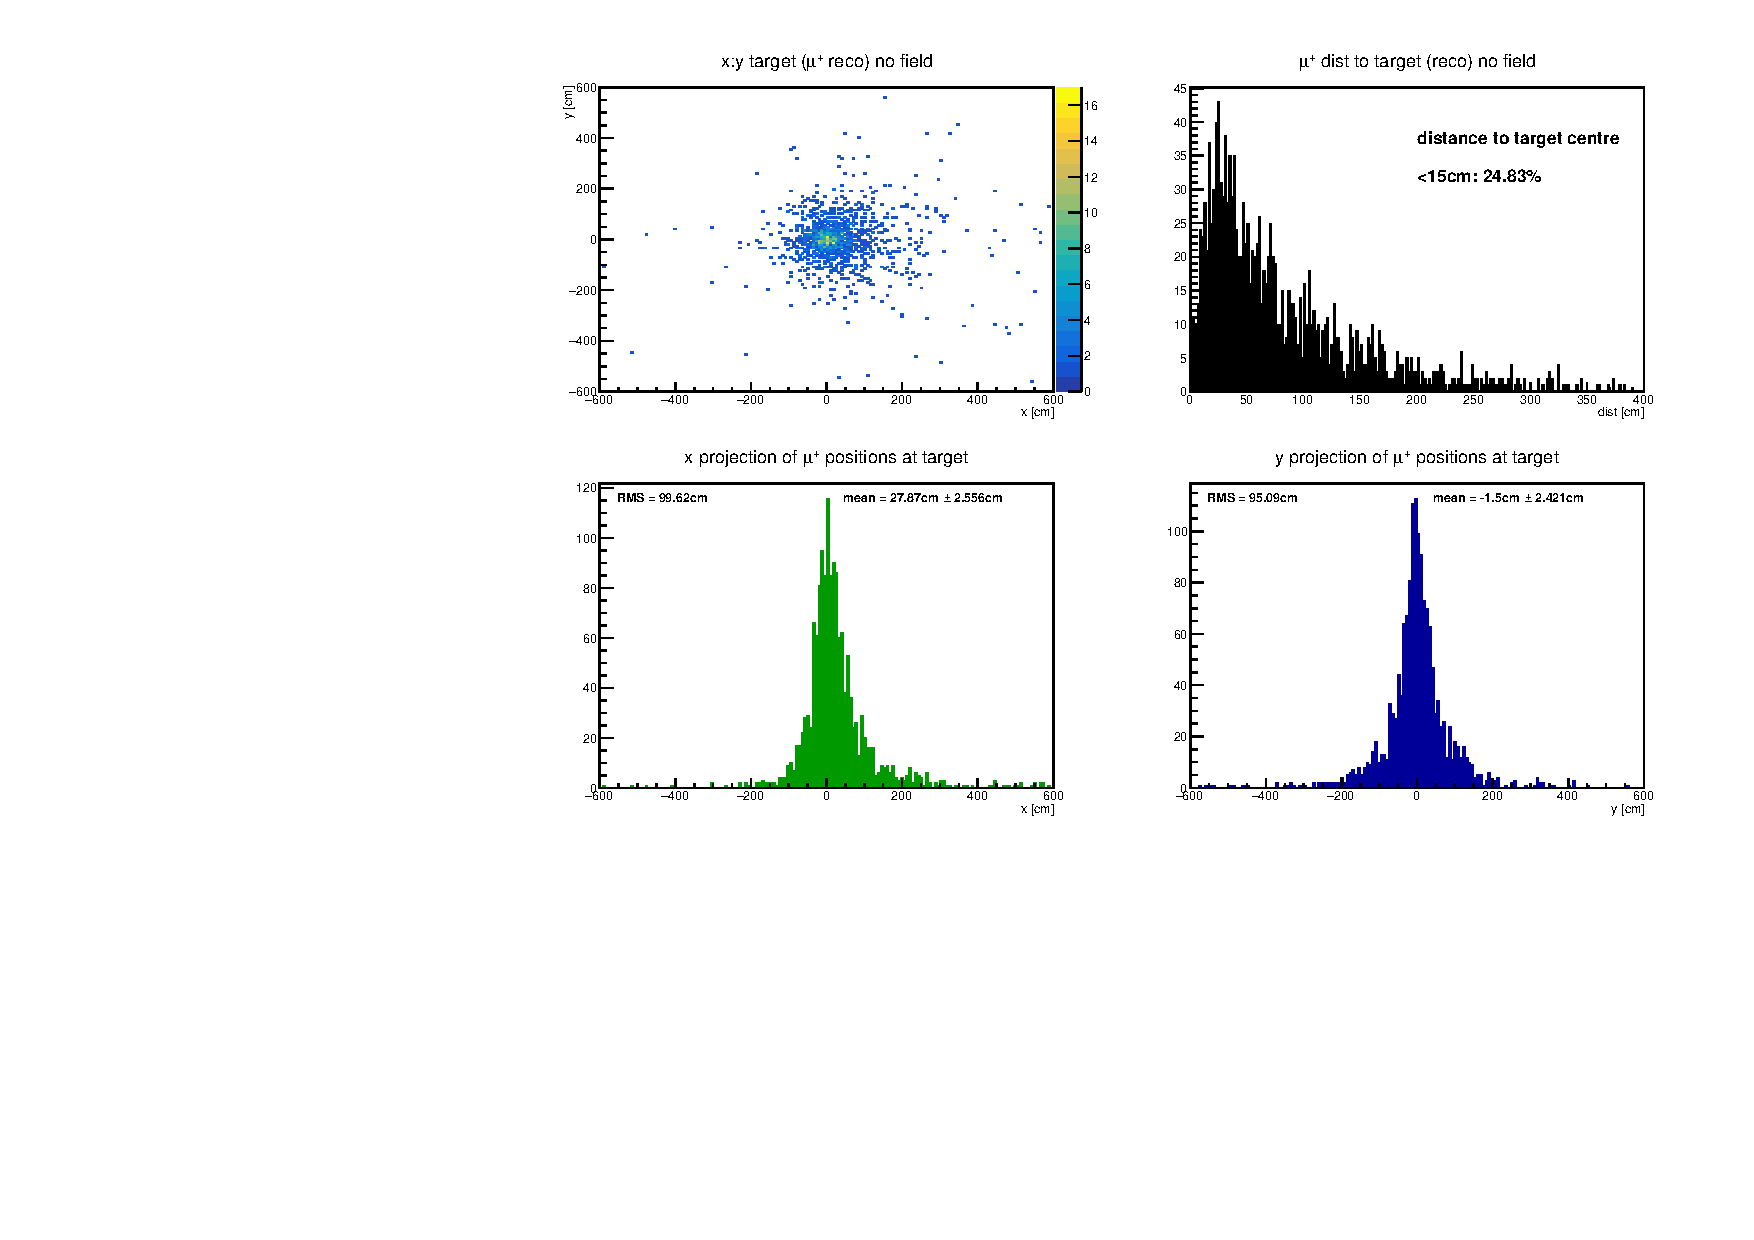
\includegraphics[width=0.5\textwidth]{../hists/nofield/1mT/target_dist_amu.pdf}
    \end{figure}
    \columnbreak
    \begin{figure}
      \centering
      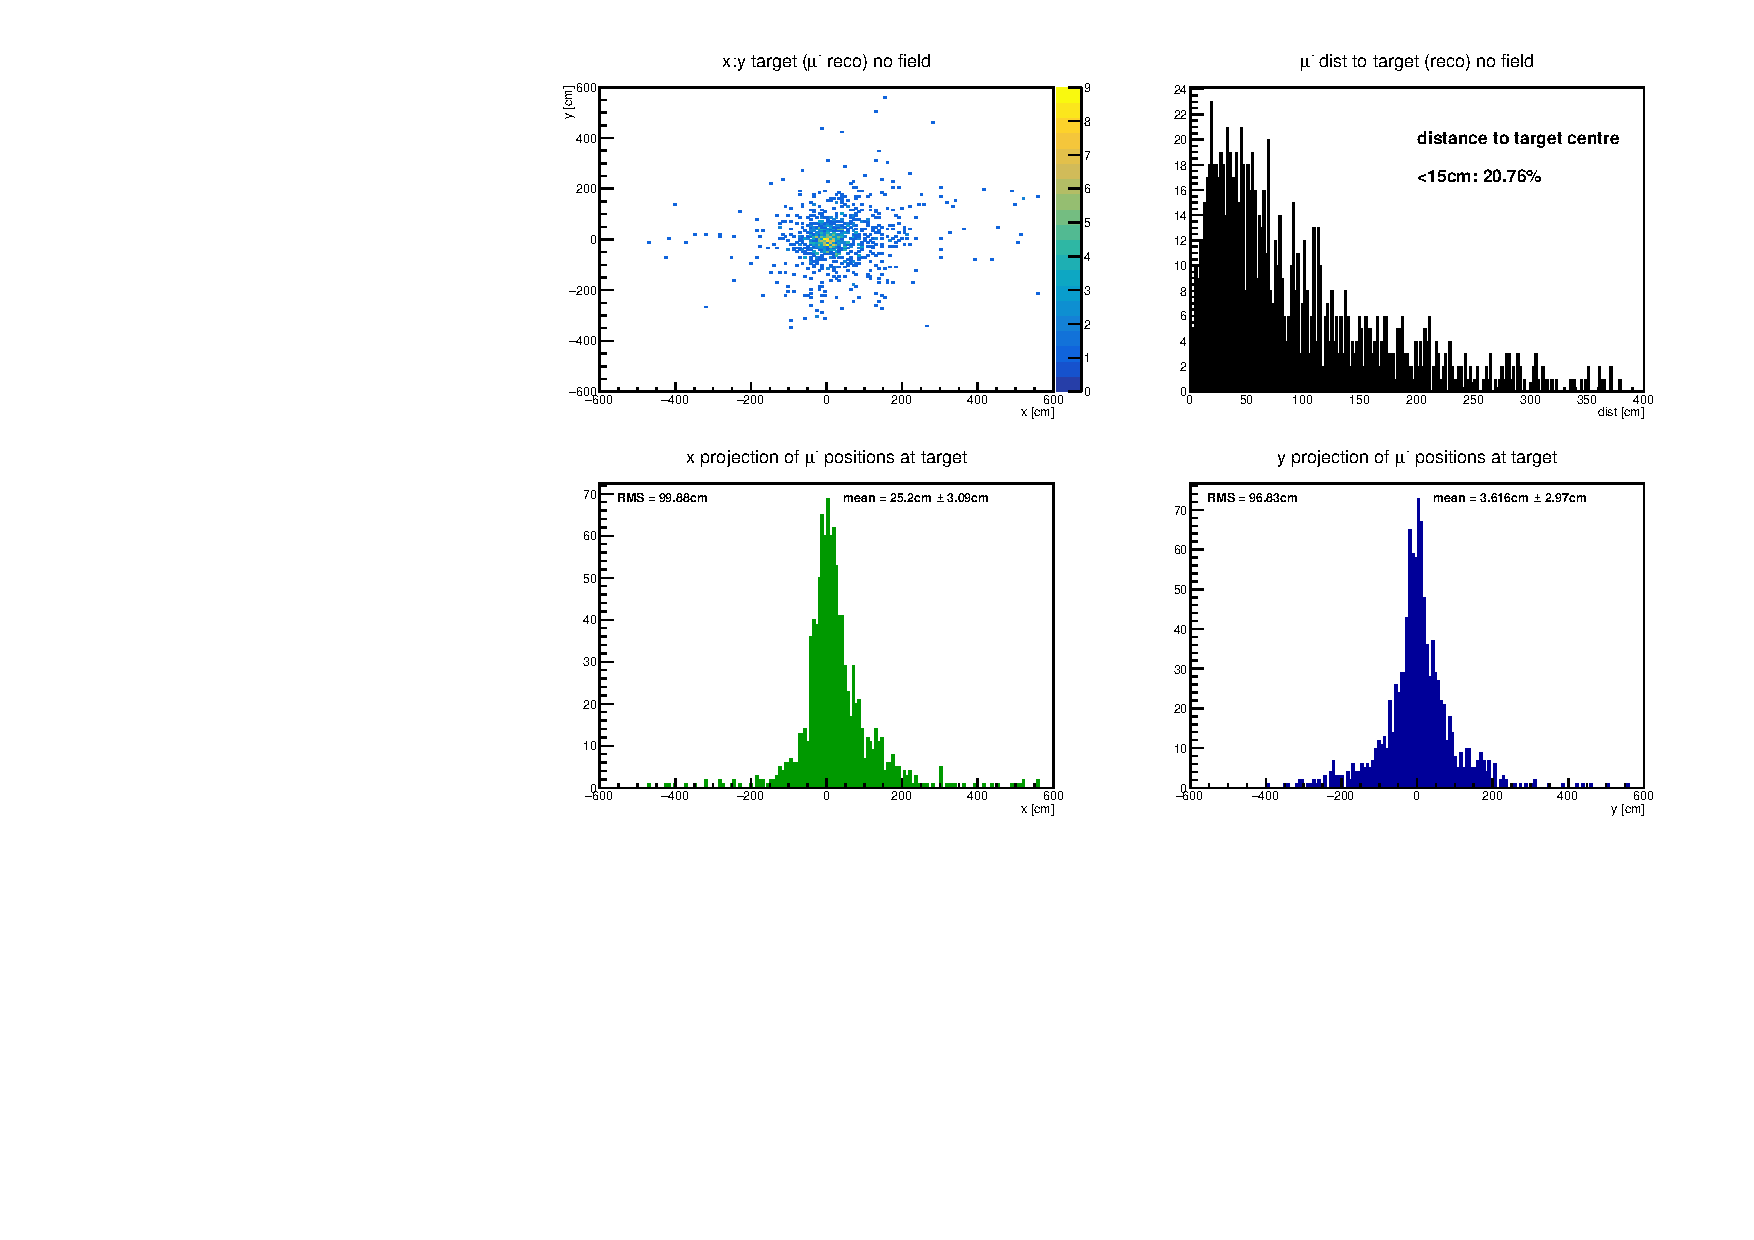
\includegraphics[width=0.5\textwidth]{../hists/nofield/1mT/target_dist_mu.pdf}
    \end{figure}
  \end{multicols}
\end{frame}

\begin{frame}
  \begin{table}
    \centering
    \begin{tabular}{c
                    S
                    S}
      \toprule
      {$\mu^{+}$} & {$B_\text{mu shield}=\SI{1}{\milli\tesla}$} & {all momenta} \\
      \midrule
      mean $x$ /cm & 27.87(256) & 23.84(238)  \\
      mean $y$ /cm & -1.5(24)   & -0.733(2356)  \\
      RMS $x$ /cm & 99.62       & 92.28  \\
      RMS $y$ /cm & 95.09       & 92.27 \\
      \midrule
      {$\mu^{-}$} & {$B_\text{mu shield}=\SI{1}{\milli\tesla}$} & {all momenta} \\
      \midrule
      mean $x$ /cm & 25.2(31) &  29.31(317)   \\
      mean $y$ /cm & 3.62(297)&  9.931(3128)  \\
      RMS $x$ /cm & 99.88     &  102.3  \\
      RMS $y$ /cm & 96.83     &  102  \\
      \bottomrule
    \end{tabular}
    \caption{Means and RMS of the reconstructed IP for no magnetic field and a $\SI{1}{\milli\tesla}$ field in the muon shield.}
    \label{tab:mean}
  \end{table}
\end{frame}

%------------------------------------------------------------------------------------------
\section{MC truth and Particle dist.}
%------------------------------------------------------------------------------------------

\begin{frame}[t]{}
  \begin{figure}
    \centering
    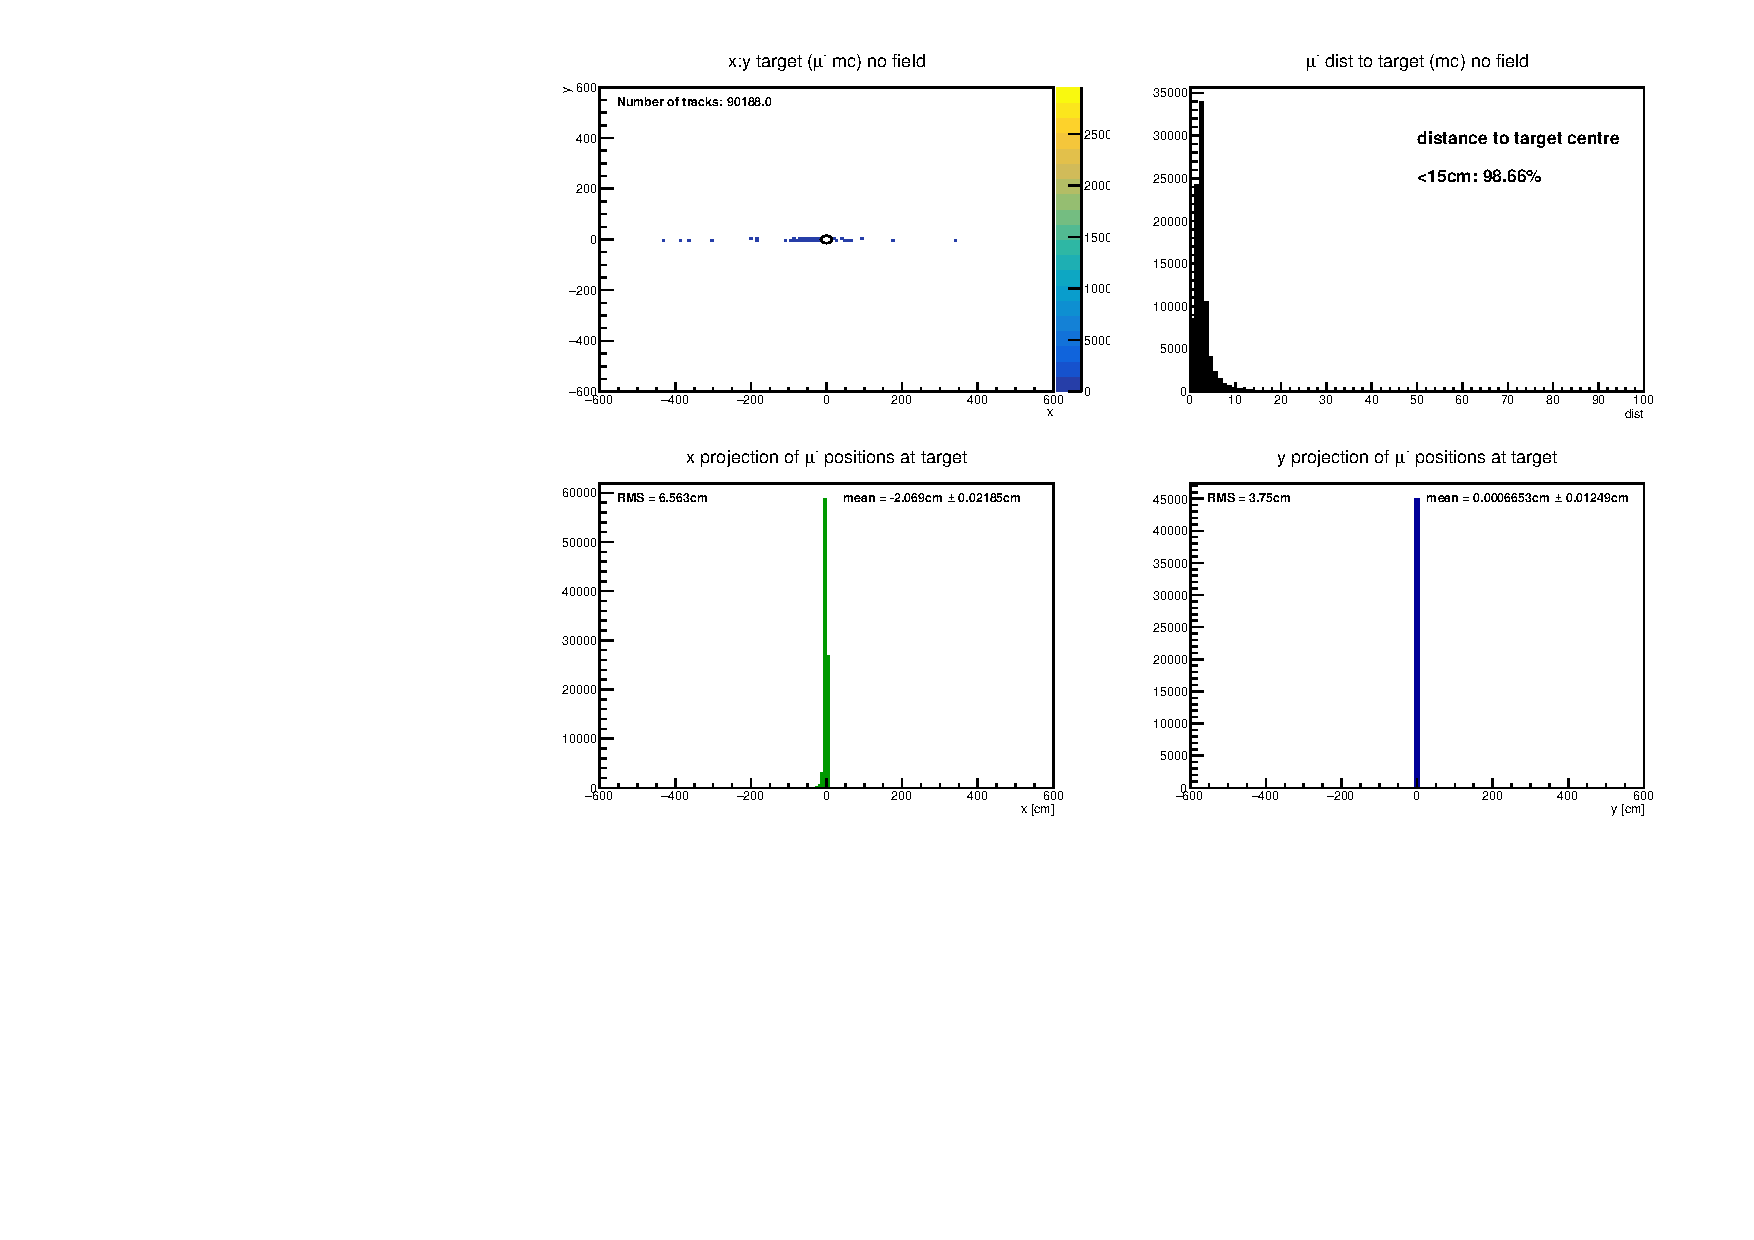
\includegraphics[width=0.65\textwidth]{../hists/nofield/p/mc_target_dist_mu.pdf}
  \end{figure}
\end{frame}



\begin{frame}[t]{}
  \begin{figure}
    \centering
    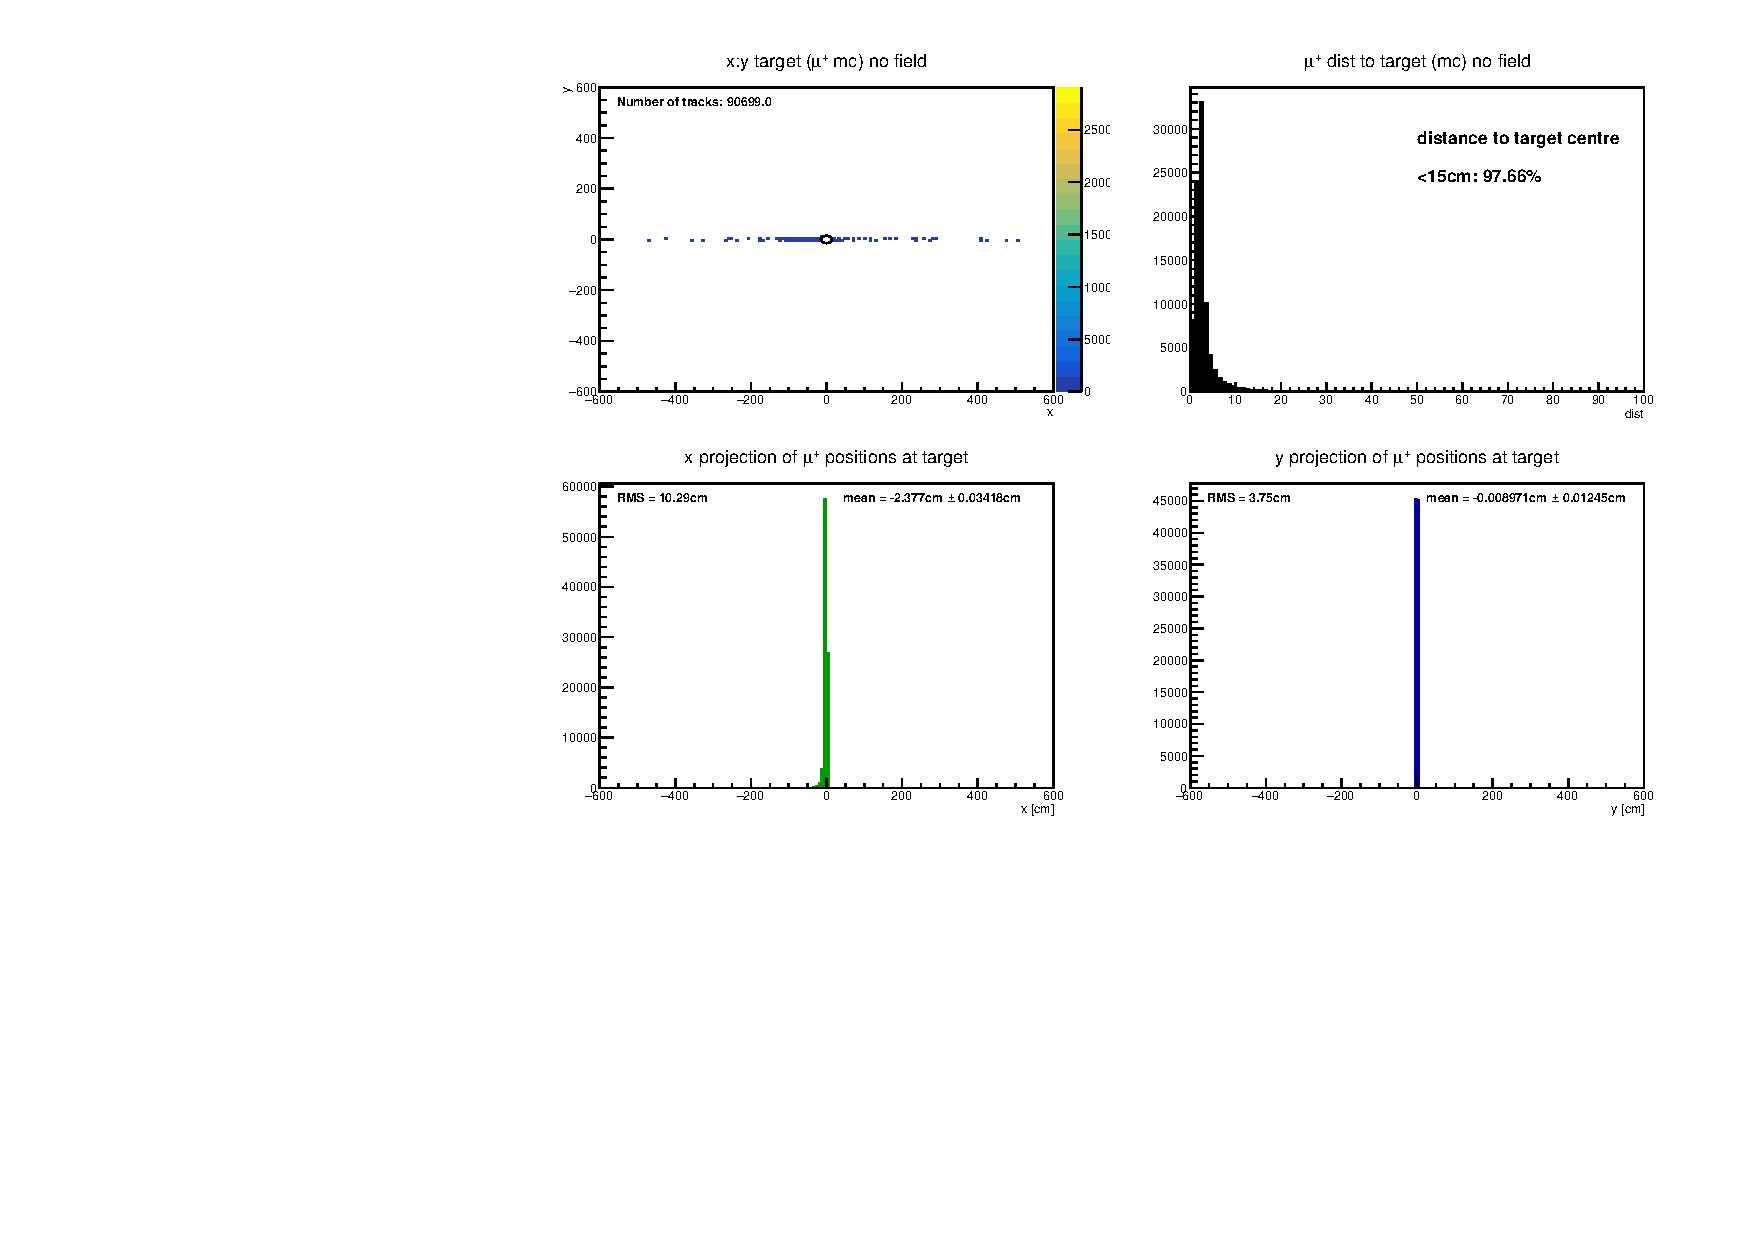
\includegraphics[width=0.65\textwidth]{../hists/nofield/p/mc_target_dist_amu.pdf}
  \end{figure}
\end{frame}

\begin{frame}[t]{}
  \begin{figure}
    \centering
    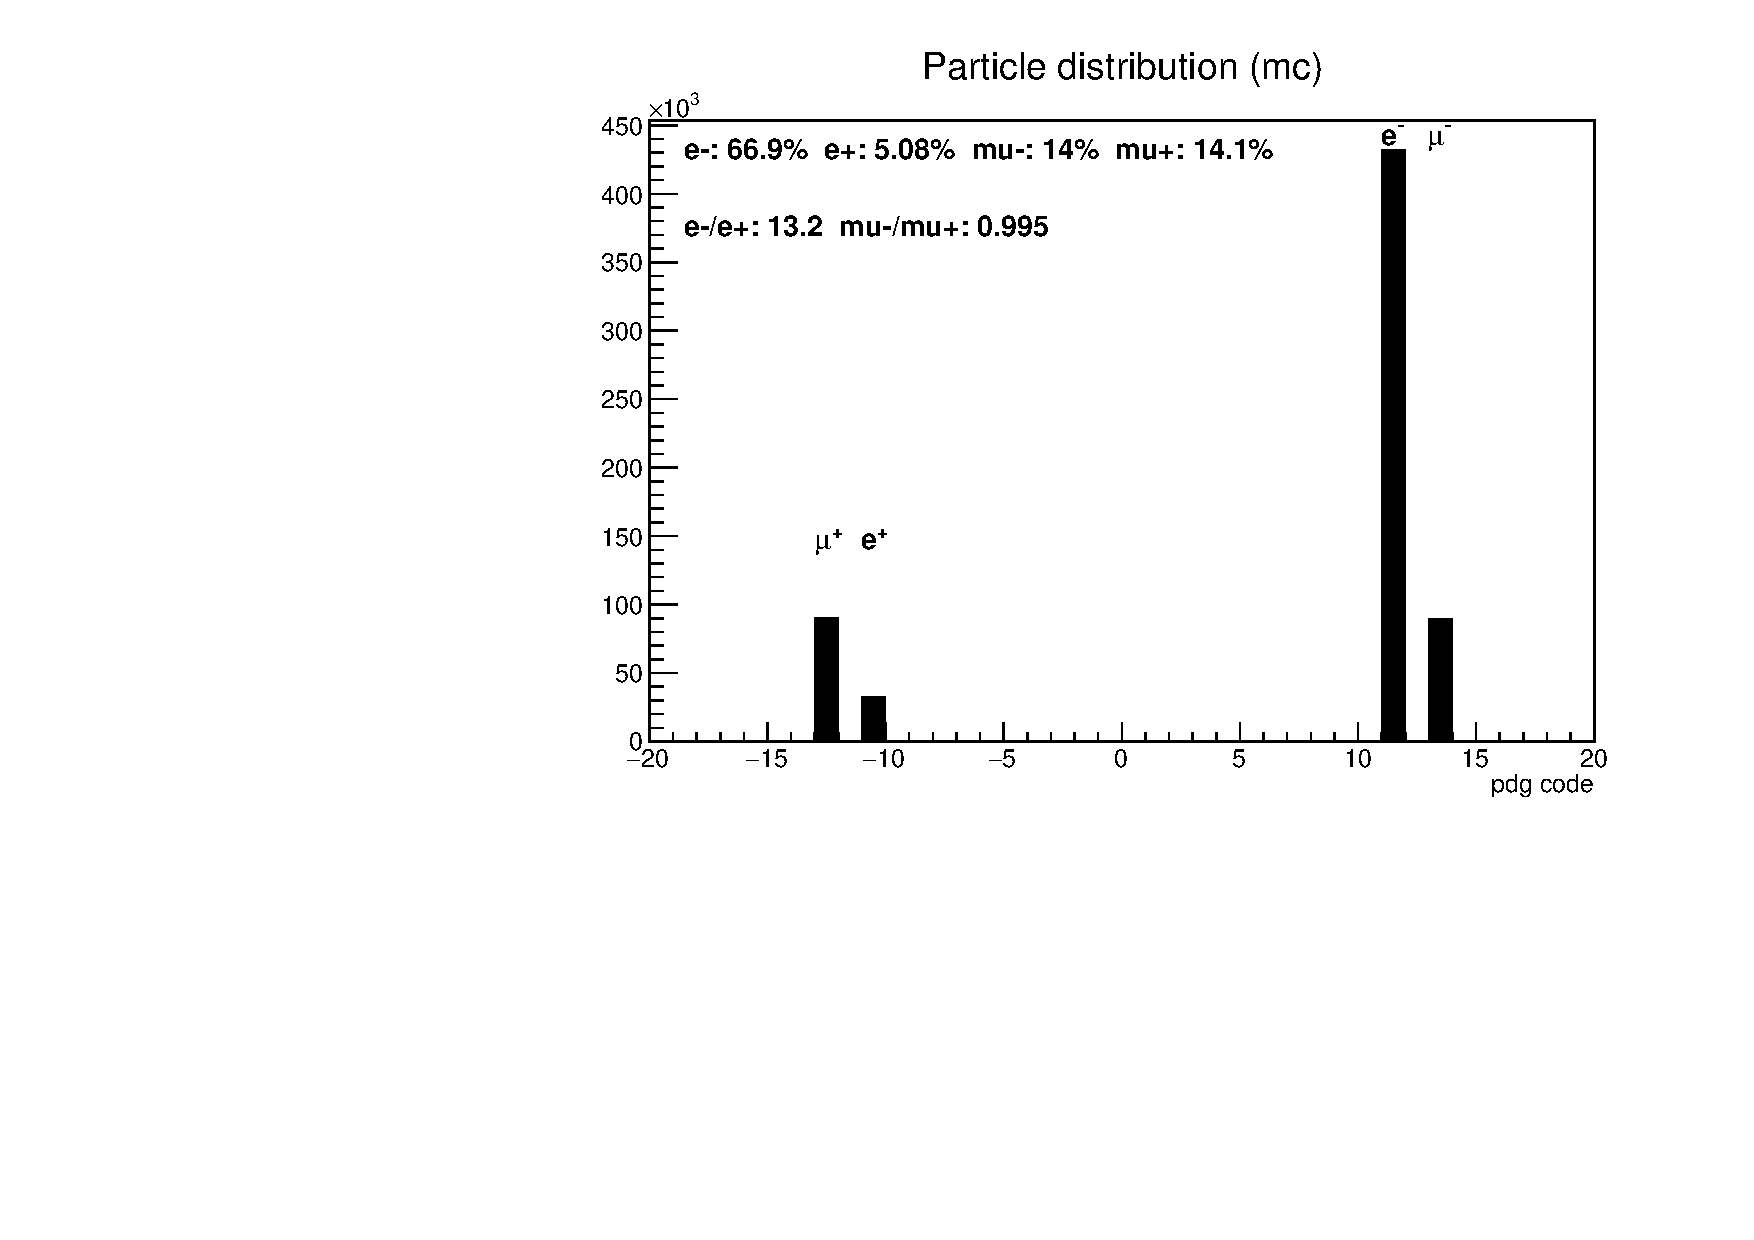
\includegraphics[width=0.65\textwidth]{../hists/nofield/allP/mc_pdg.pdf}
  \end{figure}
\end{frame}

\begin{frame}[t]{}
  \begin{figure}
    \centering
    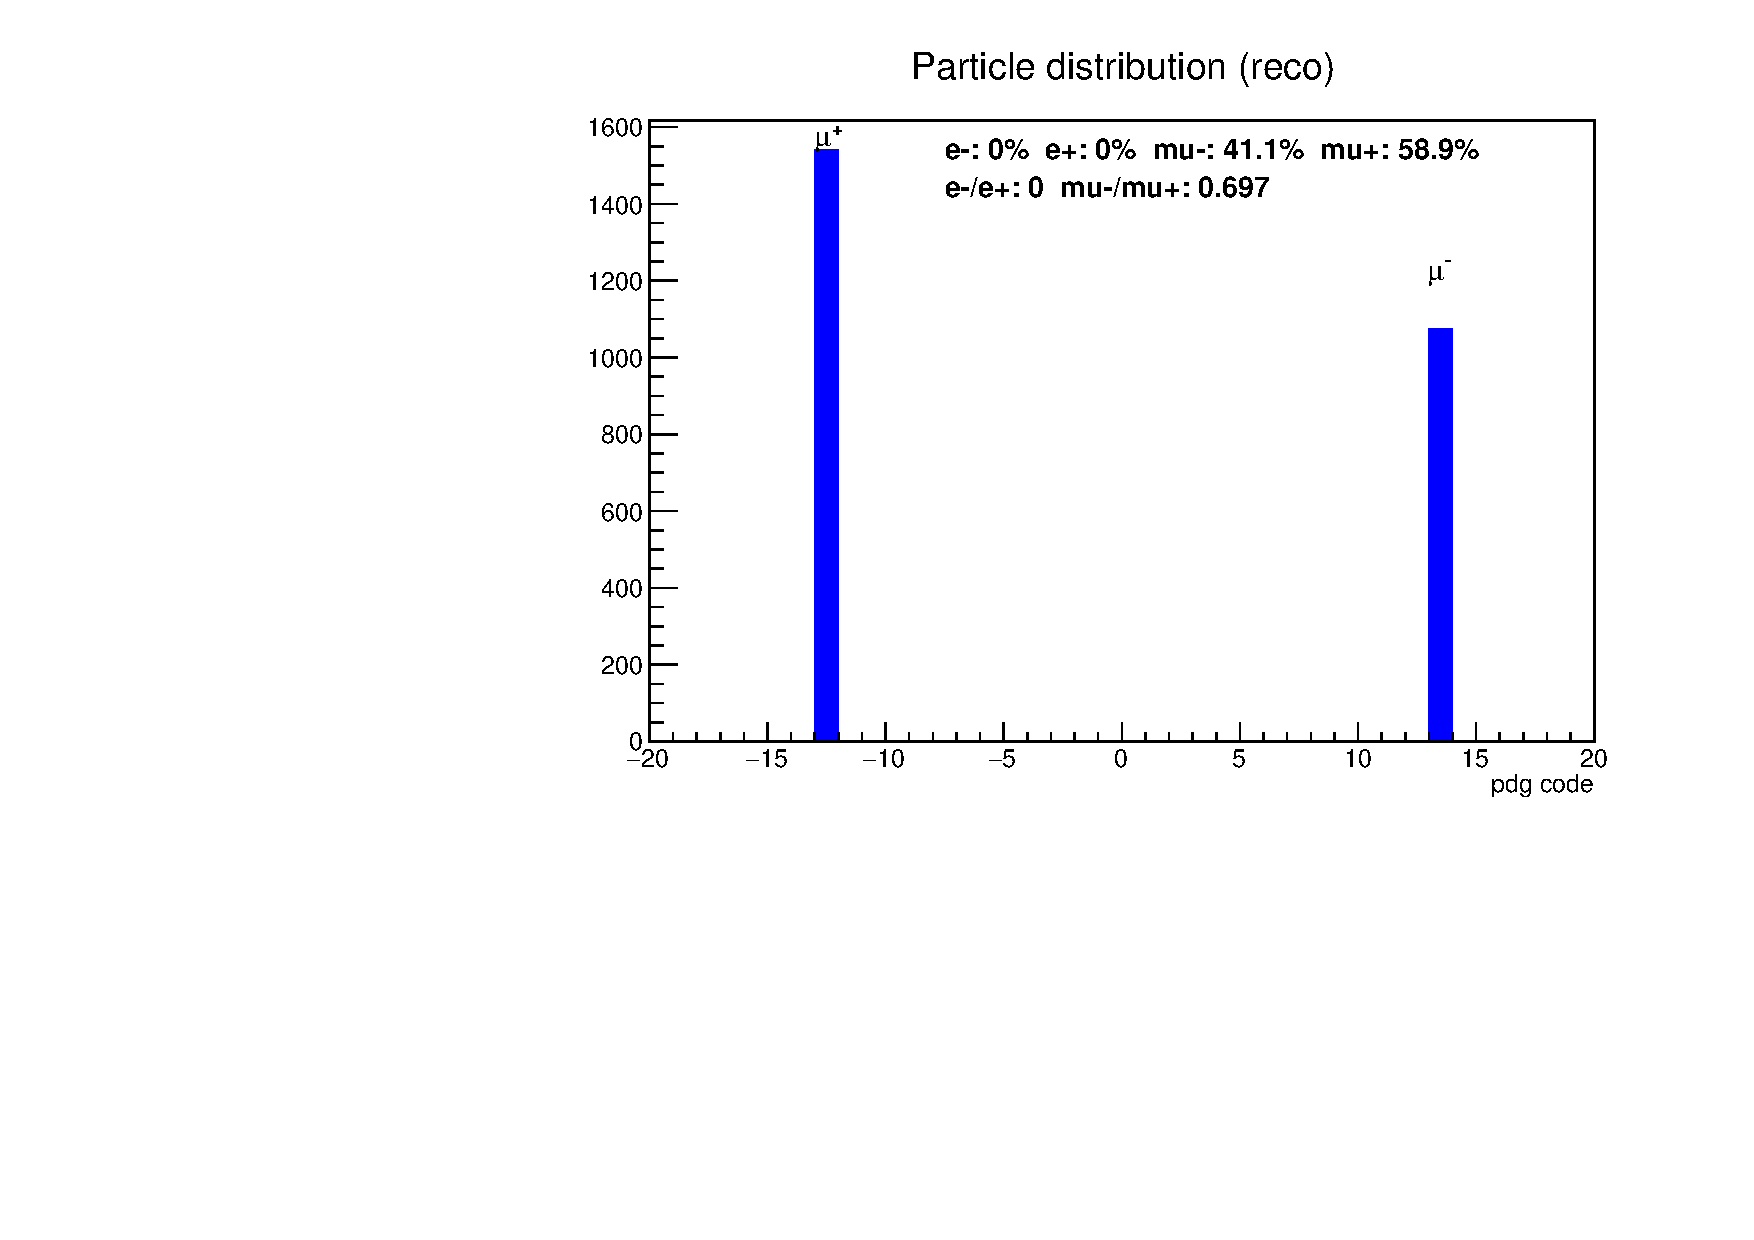
\includegraphics[width=0.65\textwidth]{../hists/nofield/allP/reco_pdg.pdf}
  \end{figure}
\end{frame}

\begin{frame}[t]{}
  \begin{itemize}
    \item When running the reconstruction script: \\
          \texttt{Error in <TDecompChol::Decompose()>: matrix not positive definite \\ Error in <TDecompChol::Solve()>: Decomposition failed} \\
    \item When trying to loop over fitted tracks in 1\,000\,000 sample: \\
          \texttt{state = track.getFittedState() \\ Exception: const genfit::MeasuredStateOnPlane\& genfit::Track::getFittedState(int id = 0, const genfit::AbsTrackRep* rep = \_\_null, bool biased = true) =>unhandled, unknown C++ exception} \\
    \item After reconstruction: \\\texttt{shipDigiReco::findVetoHitOnTrack extrapolation did not worked : 18}
  \end{itemize}
\end{frame}

\end{document}
